\chapter{Initial Value Problems}

\section{The explicit midpoint rule}

Let \(f: \R\times \R^n \rightarrow \R^n\) be a smooth mapping and consider the initial value problem 
\begin{equation}\label{ivp}
y'(t) = f(t, y(t)), \quad y(a) = y_a, \quad t\in [a,b].
\end{equation}
The {\it explicit midpoint method} (see e.g. section 4.3.3 in \cite{db})  is a method for computing an approximation to the solution of (\ref{ivp}), and it goes as follows: Let \(n\geq 1\) be an integer and \(h\coloneqq (b-a)/2n\). We then define recursively
\[
\xi_h(a) \coloneqq y_a, \quad \xi_h(a+h) \coloneqq \xi_h(a) + hf(a, \xi_h(a))
\]
and
\[
\xi_h(a + (i+1)h) \coloneqq \xi_h(a+(i-1)h) + 2hf(a+ih, \xi(a+ih)).
\]
Then \(\xi_h\) is an approximate solution to (\ref{ivp}) defined at \(a, a+h,\ldots ,b\). We are interested in the value \(X_f(h)\coloneqq \xi_h(b)\). It is shown in section 4.3.3. in \cite{db} that \(X_f(h)\) has an asymptotic expansion in \(h^2\). We have the following implementation in Python of the explicit midpoint rule for computing \(X_f(h)\).

\begin{minted}[tabsize=2, fontsize=\footnotesize]{python}
class ExplicitMidpointRule(Scheme):

	def __init__(self):
		super(ExplicitMidpointRule, self).__init__(2)

	def apply(self, ivp, n):
		h = (ivp.b - ivp.a) / (2 * n)
		y_sl = ivp.y0
		y_l = ivp.y0 + h * ivp.f(ivp.a, ivp.y0)

		for i in range(1, 2 * n):
			tmp = y_l
			y_l = y_sl + 2 * h * ivp.f(ivp.a + i * h, y_l)
			y_sl = tmp

		return y_l
\end{minted}

\section{Numerical experiments}

In this section we are going to extrapolate the explicit midpoint rule and analyze the convergence of the approximations as we extrapolate more often. Consider the initial value problem (\ref{ivp}). Let \(n_1 < n_2 < \cdots\) be some sequence of integers and \(h_i \coloneqq (b-a) / n_i\). Let \(X_{ij}\) the extrapolation table which we get from extrapolating in \(h^2\), using the points \((h_i,X_f(h_i))\). Let \(\varepsilon_i \coloneqq |X_{ii} - y(b)|\) be the absolute error. We are going to do the same convergence and efficency analysis as in the two previous chapters. We will both do the computations using high precision arithmetic with \(500\) correct digits and also in standard double precision.\\

In those cases where we do not have an analytic solution to the equations, we computed a reference solution up to high precision. We did that by using extrapolation with the harmonic sequence and estimating the error as the difference between successive terms in the sequence of approximations.\\

Now we will consider the results of the experiments.

\subsection{Exponential growth}
First we will consider the following initial value problem:
\begin{equation}\label{42}
y'(x) = y(x),\quad y(0) = 1, \quad x\in [0,1]
\end{equation}
whose solution is the analytic function \(y(x) = e^x\).

\begin{figure}[H]
\centering
\begin{minipage}{0.45\textwidth}
\centering
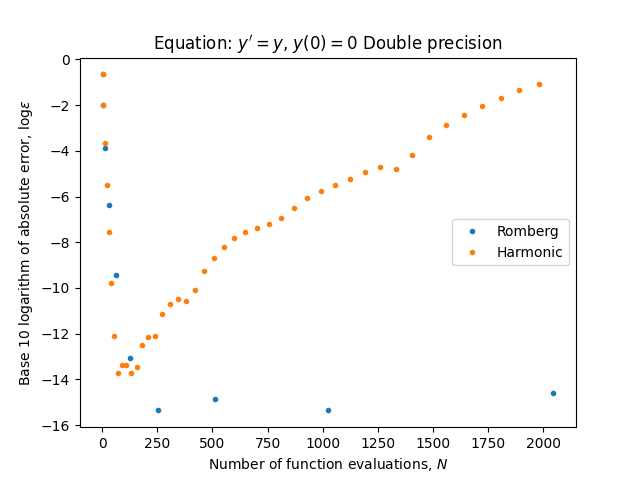
\includegraphics[scale=0.45]{../results/emr_plots/exp_growth.png}
\end{minipage}
\begin{minipage}{0.45\textwidth}
\centering
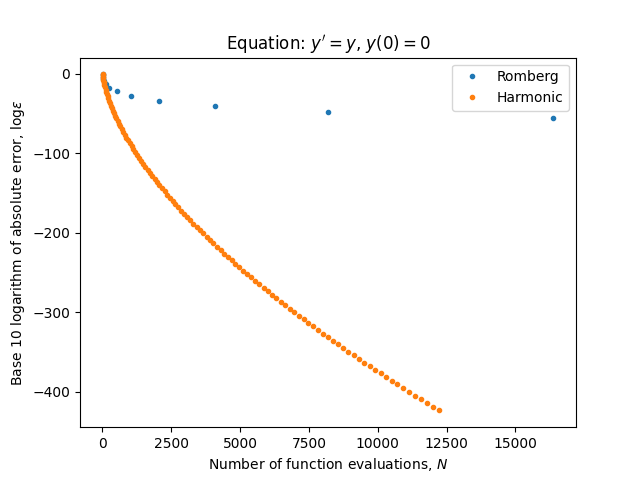
\includegraphics[scale=0.45]{../results/emr_plots/exp_growth_hp.png}
\end{minipage}
\end{figure}

\begin{figure}[H]
\centering
\begin{minipage}{0.45\textwidth}
\centering
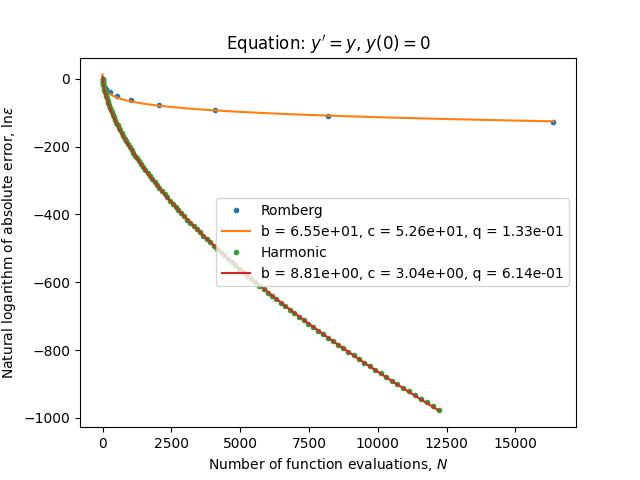
\includegraphics[scale=0.45]{../results/emr_plots/exp_growth_hp_trend.png}
\end{minipage}
\begin{minipage}{0.45\textwidth}
\centering
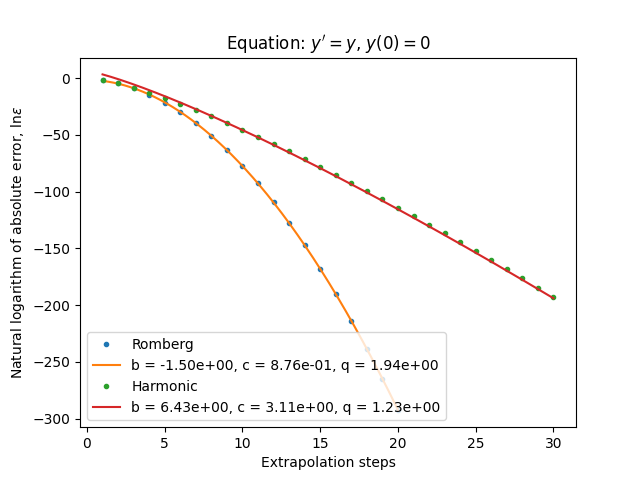
\includegraphics[scale=0.45]{../results/emr_plots/exp_growth_hp_steps.png}
\end{minipage}
\end{figure}

\begin{figure}[H]
\centering
\begin{minipage}{0.45\textwidth}
\centering
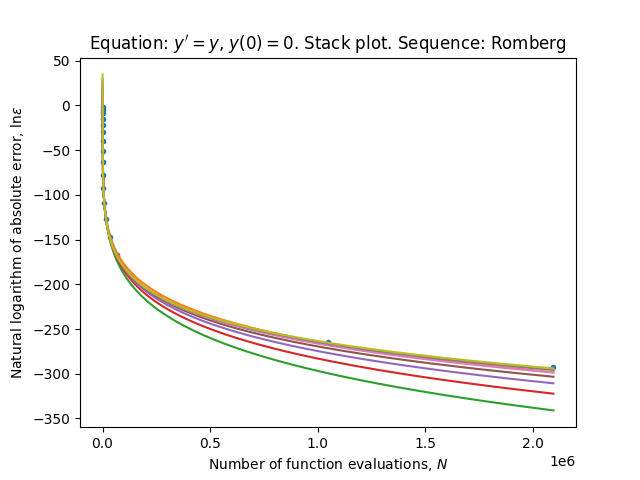
\includegraphics[scale=0.45]{../results/emr_plots/exp_growth_hp_romberg_stack.png}
\end{minipage}
\begin{minipage}{0.45\textwidth}
\centering
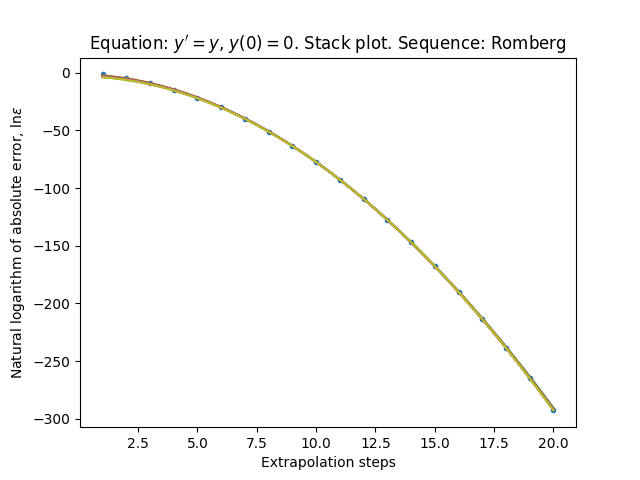
\includegraphics[scale=0.45]{../results/emr_plots/exp_growth_hp_romberg_steps_stack.png}
\end{minipage}
\end{figure}

\begin{figure}[H]
\centering
\begin{minipage}{0.45\textwidth}
\centering
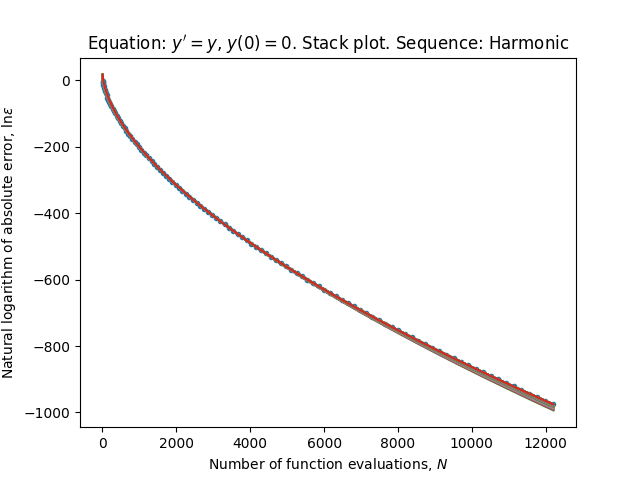
\includegraphics[scale=0.45]{../results/emr_plots/exp_growth_hp_harmonic_stack.png}
\end{minipage}
\begin{minipage}{0.45\textwidth}
\centering
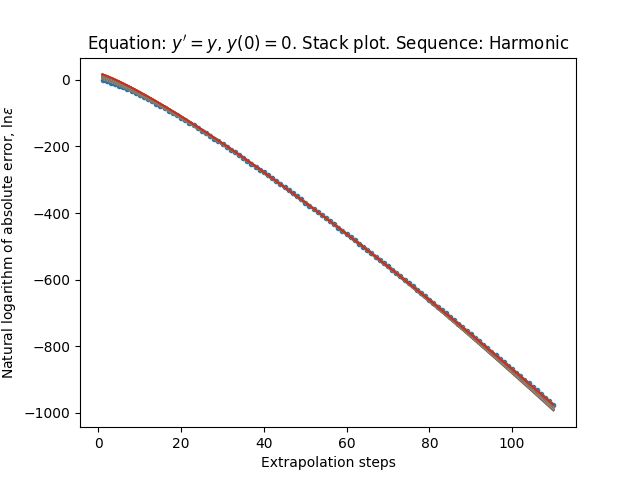
\includegraphics[scale=0.45]{../results/emr_plots/exp_growth_hp_harmonic_steps_stack.png}
\end{minipage}
\end{figure}

\begin{table}[H]
    \centering
    \small
    \begin{tabular}{c||c|c|c|c|c|c|c|c}
Plot & \(A\)-mean & \(A\)-var & \(c\)-mean & \(c\)-var & \(q\)-mean & \(q\)-var & \(\rho_{\operatorname{lin}}\) & \(\rho_{\ln}\)\\\hline
\rowcolor{red}
RS-evals & \(6.2[+65]\) & \(6.0[+00]\) & \(7.2[+01]\) & \(1.2[-01]\) & \(1.2[-01]\) & \(3.1[-02]\) & \(1.4[+08]\) & \(6.9[-04]\) \\
\rowcolor{yellow}
HS-evals & \(1.2[+09]\) & \(6.4[+00]\) & \(3.3[+00]\) & \(5.2[-03]\) & \(6.1[-01]\) & \(1.7[-04]\) & \(8.4[+04]\) & \(5.6[-06]\) \\
\rowcolor{green}
RS-steps & \(8.7[-02]\) & \(2.2[-01]\) & \(8.4[-01]\) & \(9.2[-04]\) & \(1.9[+00]\) & \(2.8[-05]\) & \(3.3[-01]\) & \(4.5[-06]\) \\
\rowcolor{yellow}
HS-steps & \(3.8[+07]\) & \(6.0[+00]\) & \(3.3[+00]\) & \(4.5[-03]\) & \(1.2[+00]\) & \(1.4[-04]\) & \(1.6[+04]\) & \(4.5[-06]\) \\
    \end{tabular}
    \label{tab:my_label}
\end{table}

The Harmonic sequence performes better. We get down to machine level precision using either sequence in double precision arithmetic.\\

We clearly have exponential convergence in the number of steps for the Romberg sequence and the fitting for the Harmonic sequence seems nice but we though have very big values for \(A\).

\subsection{Logistic curve}

Then we will consider the following initial value problem
\begin{equation}\label{43}
y'(x) = y(x)(1-y(x)),\quad y(0) = 1/2, \quad x\in [0,1]
\end{equation}

whose solution is the sigmoid function
\[
\sigma(x) = \frac{1}{1 + e^{-x}}
\]
which is analytic.

\begin{figure}[H]
\centering
\begin{minipage}{0.45\textwidth}
\centering
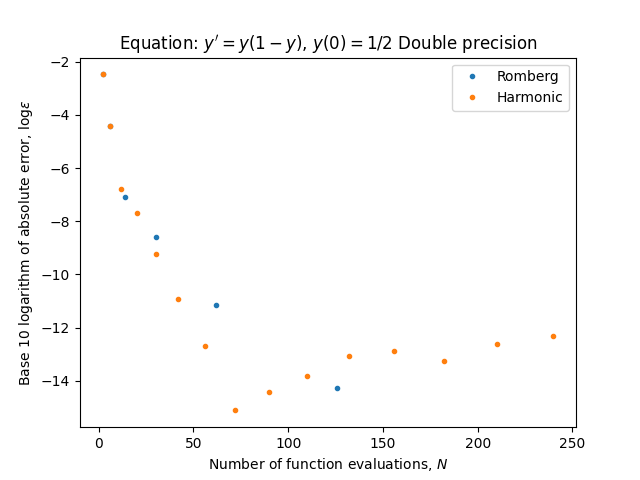
\includegraphics[scale=0.45]{../results/emr_plots/logistic.png}
\end{minipage}
\begin{minipage}{0.45\textwidth}
\centering
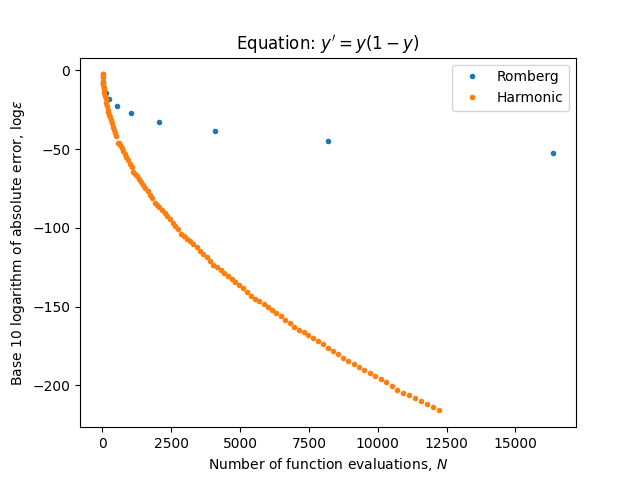
\includegraphics[scale=0.45]{../results/emr_plots/logistic_hp.png}
\end{minipage}
\end{figure}

\begin{figure}[H]
\centering
\begin{minipage}{0.45\textwidth}
\centering
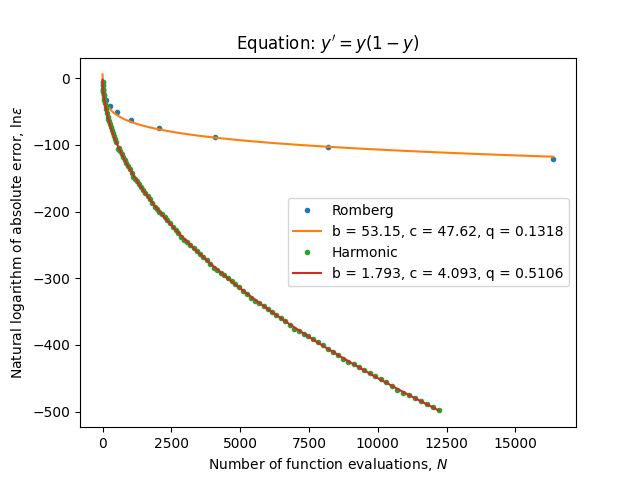
\includegraphics[scale=0.45]{../results/emr_plots/logistic_hp_trend.png}
\end{minipage}
\begin{minipage}{0.45\textwidth}
\centering
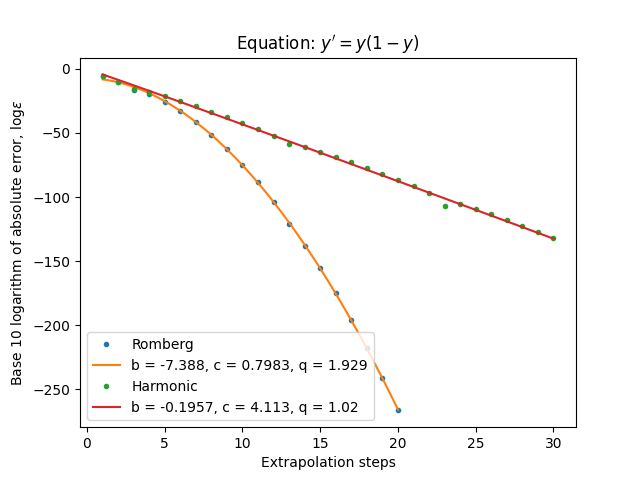
\includegraphics[scale=0.45]{../results/emr_plots/logistic_hp_steps.png}
\end{minipage}
\end{figure}

\begin{figure}[H]
\centering
\begin{minipage}{0.45\textwidth}
\centering
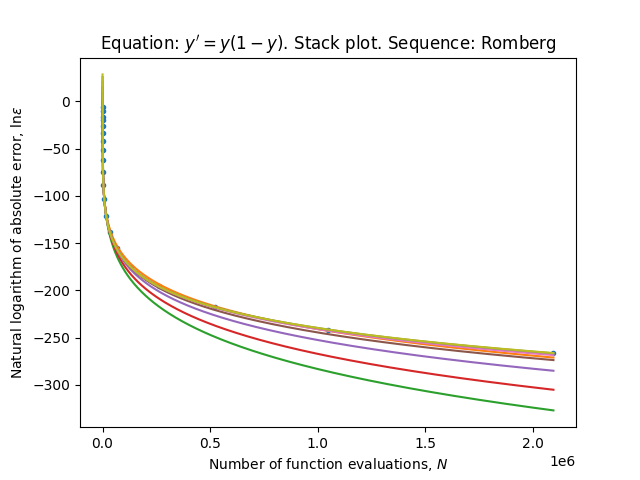
\includegraphics[scale=0.45]{../results/emr_plots/logistic_hp_romberg_stack.png}
\end{minipage}
\begin{minipage}{0.45\textwidth}
\centering
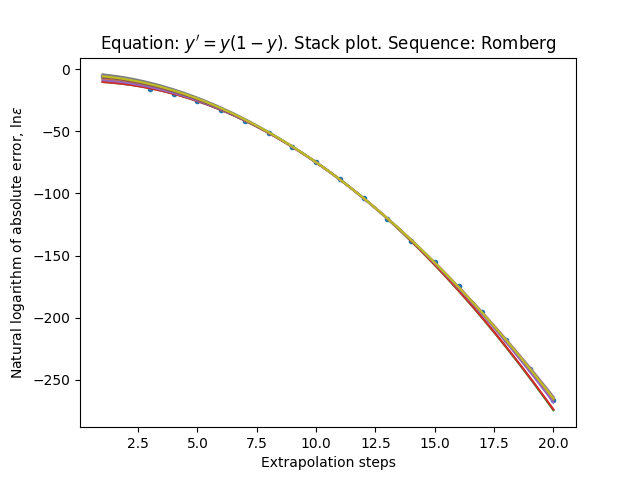
\includegraphics[scale=0.45]{../results/emr_plots/logistic_hp_romberg_steps_stack.png}
\end{minipage}
\end{figure}

\begin{figure}[H]
\centering
\begin{minipage}{0.45\textwidth}
\centering
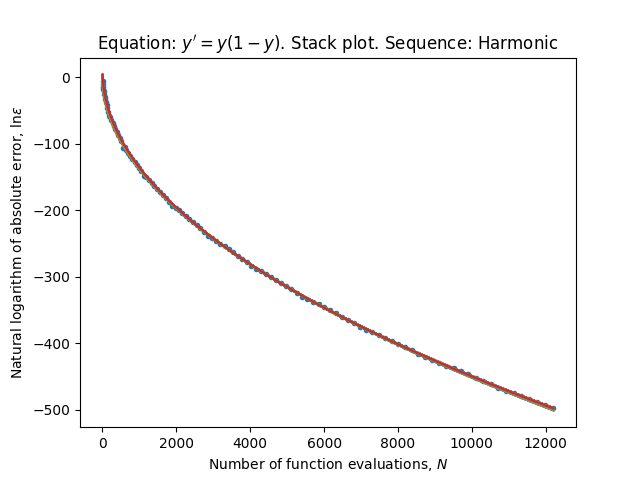
\includegraphics[scale=0.45]{../results/emr_plots/logistic_hp_harmonic_stack.png}
\end{minipage}
\begin{minipage}{0.45\textwidth}
\centering
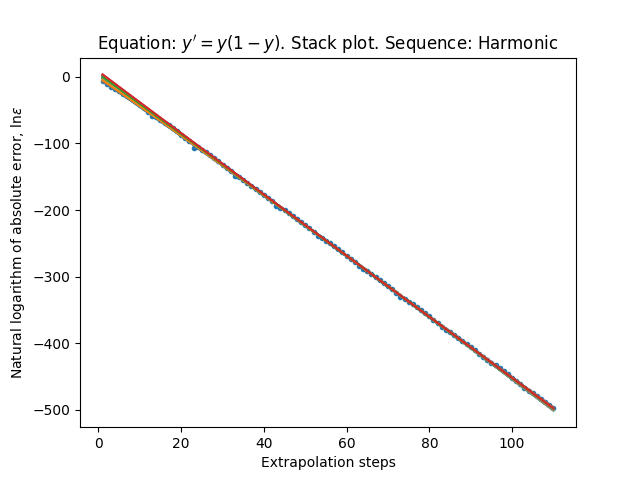
\includegraphics[scale=0.45]{../results/emr_plots/logistic_hp_harmonic_steps_stack.png}
\end{minipage}
\end{figure}

\begin{table}[H]
    \centering
    \small
    \begin{tabular}{c||c|c|c|c|c|c|c|c}
Plot & \(A\)-mean & \(A\)-var & \(c\)-mean & \(c\)-var & \(q\)-mean & \(q\)-var & \(\rho_{\operatorname{lin}}\) & \(\rho_{\ln}\)\\\hline
\rowcolor{red}
RS-evals & \(8.8[+63]\) & \(6.0[+00]\) & \(7.1[+01]\) & \(2.0[-01]\) & \(1.2[-01]\) & \(6.4[-02]\) & \(6.4[+05]\) & \(6.1[-04]\) \\
\rowcolor{green}
HS-evals & \(2.5[+03]\) & \(9.4[+00]\) & \(4.2[+00]\) & \(3.6[-03]\) & \(5.1[-01]\) & \(1.3[-04]\) & \(1.9[+01]\) & \(1.3[-05]\) \\
\rowcolor{green}
RS-steps & \(1.0[-02]\) & \(1.9[+00]\) & \(8.1[-01]\) & \(3.1[-02]\) & \(1.9[+00]\) & \(1.1[-03]\) & \(8.4[-01]\) & \(4.6[-05]\) \\
\rowcolor{green}
HS-steps & \(2.6[+02]\) & \(9.2[+00]\) & \(4.3[+00]\) & \(3.5[-03]\) & \(1.0[+00]\) & \(1.3[-04]\) & \(9.3[+00]\) & \(1.3[-05]\) \\
    \end{tabular}
    \label{tab:my_label}
\end{table}

The harmonic sequence performes better and we get down to machine level precisision using either sequence, in double precision.\\

We seem to have exponential convergence in the number of steps for the Romberg sequence and the models fit well for the harmonic sequence.\\

\subsection{Tangens}

Now we will consider the following equation
\begin{equation}
y'(x) = 1 + y(x)^2, \quad y(0) = 0,\quad x\in [0,1]
\end{equation}

whose solution is 
\[
y(x) \coloneqq \tan(x)
\]
which is meromorphic and we are quite far from singularites.

\begin{figure}[H]
\centering
\begin{minipage}{0.45\textwidth}
\centering
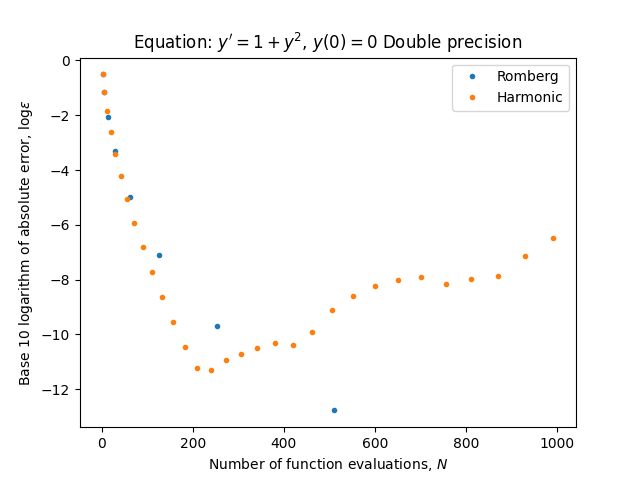
\includegraphics[scale=0.45]{../results/emr_plots/tangens.png}
\end{minipage}
\begin{minipage}{0.45\textwidth}
\centering
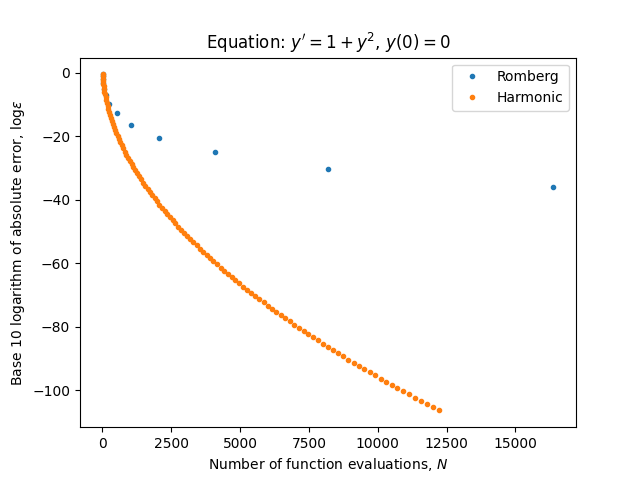
\includegraphics[scale=0.45]{../results/emr_plots/tangens_hp.png}
\end{minipage}
\end{figure}

\begin{figure}[H]
\centering
\begin{minipage}{0.45\textwidth}
\centering
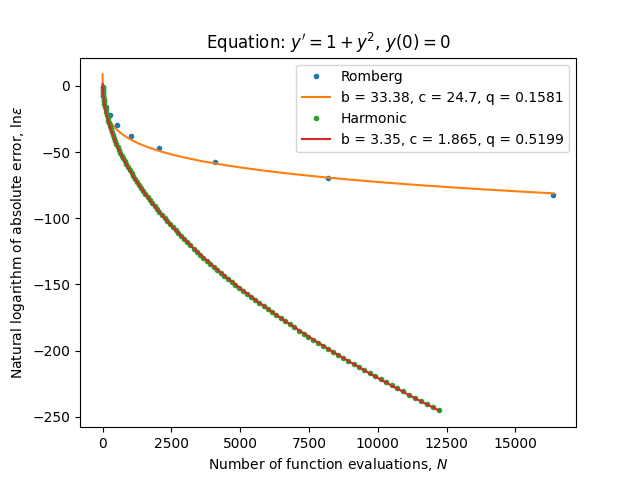
\includegraphics[scale=0.45]{../results/emr_plots/tangens_hp_trend.png}
\end{minipage}
\begin{minipage}{0.45\textwidth}
\centering
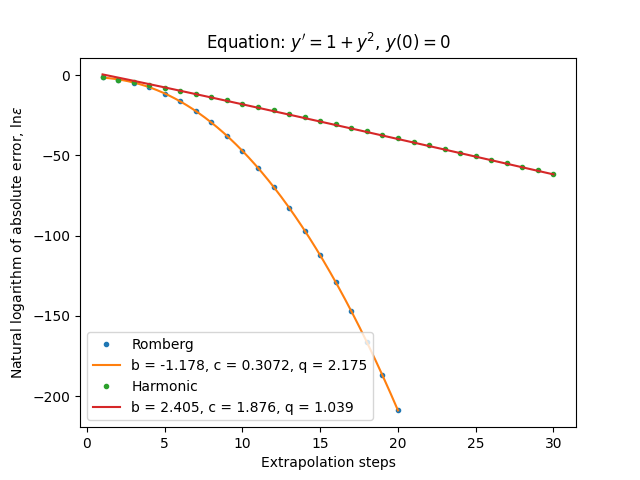
\includegraphics[scale=0.45]{../results/emr_plots/tangens_hp_steps.png}
\end{minipage}
\end{figure}

\begin{figure}[H]
\centering
\begin{minipage}{0.45\textwidth}
\centering
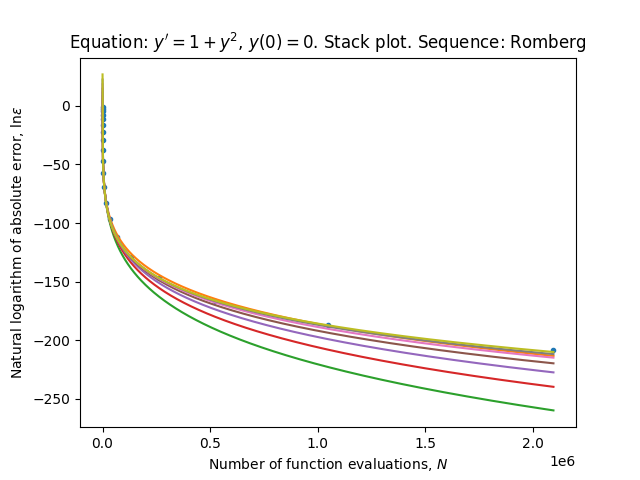
\includegraphics[scale=0.45]{../results/emr_plots/tangens_hp_romberg_stack.png}
\end{minipage}
\begin{minipage}{0.45\textwidth}
\centering
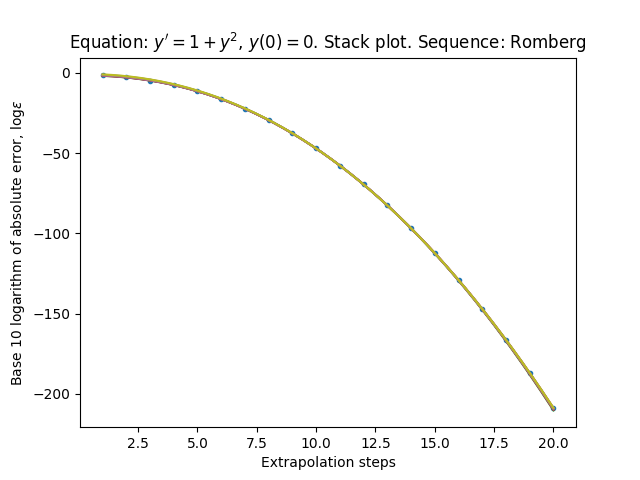
\includegraphics[scale=0.45]{../results/emr_plots/tangens_hp_romberg_steps_stack.png}
\end{minipage}
\end{figure}

\begin{figure}[H]
\centering
\begin{minipage}{0.45\textwidth}
\centering
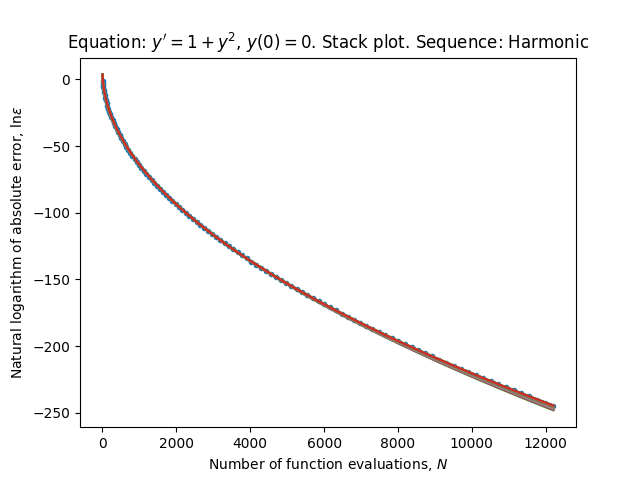
\includegraphics[scale=0.45]{../results/emr_plots/tangens_hp_harmonic_stack.png}
\end{minipage}
\begin{minipage}{0.45\textwidth}
\centering
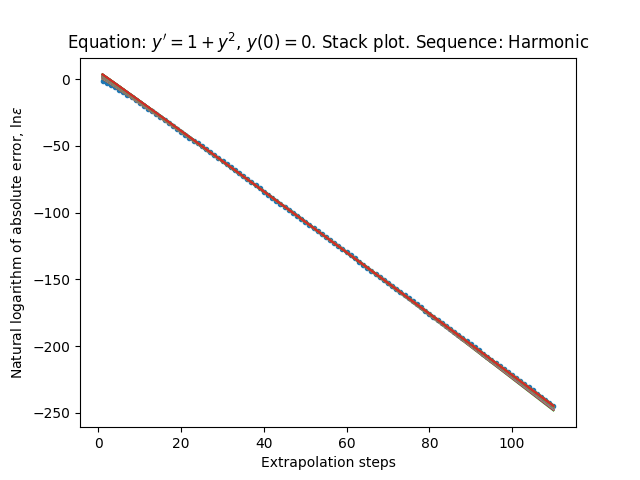
\includegraphics[scale=0.45]{../results/emr_plots/tangens_hp_harmonic_steps_stack.png}
\end{minipage}
\end{figure}

\begin{table}[H]
    \centering
    \small
    \begin{tabular}{c||c|c|c|c|c|c|c|c}
Plot & \(A\)-mean & \(A\)-var & \(c\)-mean & \(c\)-var & \(q\)-mean & \(q\)-var & \(\rho_{\operatorname{lin}}\) & \(\rho_{\ln}\)\\\hline
\rowcolor{red}
RS-evals & \(9.5[+36]\) & \(6.0[+00]\) & \(3.3[+01]\) & \(1.7[-01]\) & \(1.5[-01]\) & \(3.6[-02]\) & \(1.1[+06]\) & \(9.5[-04]\) \\
\rowcolor{green}
HS-evals & \(3.6[+02]\) & \(5.7[-01]\) & \(2.0[+00]\) & \(2.5[-03]\) & \(5.1[-01]\) & \(1.1[-04]\) & \(2.8[+01]\) & \(5.9[-06]\) \\
\rowcolor{green}
RS-steps & \(3.5[-01]\) & \(1.1[-01]\) & \(3.0[-01]\) & \(1.0[-03]\) & \(2.2[+00]\) & \(2.6[-05]\) & \(6.7[-02]\) & \(1.3[-06]\) \\
\rowcolor{green}
HS-steps & \(1.2[+02]\) & \(5.4[-01]\) & \(2.0[+00]\) & \(2.3[-03]\) & \(1.0[+00]\) & \(1.0[-04]\) & \(2.0[+01]\) & \(5.3[-06]\) \\
    \end{tabular}
    \label{tab:my_label}
\end{table}

The harmonic sequence performes better and we get down to machine level precision in double precision arithmetic, using either sequence.\\

Here we clearly have exponential convergence in the number of steps for the Romberg sequence and the fit is also very nice for the harmonic sequence.

\subsection{The logarithm}

Now we will consider the following initial value problem:

\begin{equation}
y'(t) = \exp(-y(t)), \quad y(0) = \ln(a), \quad t\in [0,1].
\end{equation}

whose solution is 

\[
y(t) = \ln(a + t).
\]

The solution is analytic on but with a singularity on the closed horizontal ray from \(-a\) to \(-\infty\).

\subsubsection{\(a = 1\)}

\begin{figure}[H]
\centering
\begin{minipage}{0.45\textwidth}
\centering
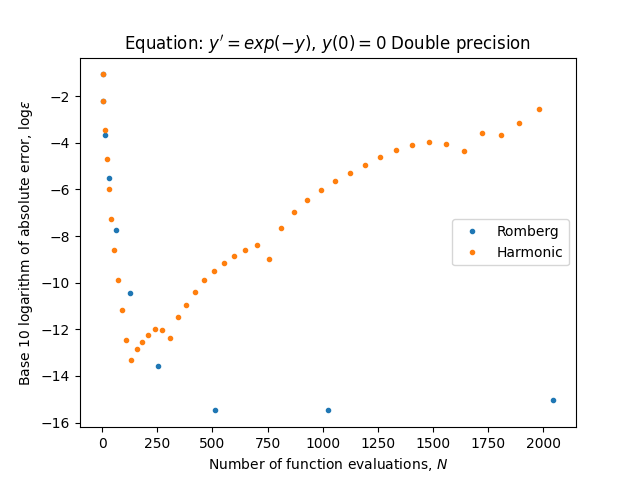
\includegraphics[scale=0.45]{../results/emr_plots/ln_e0.png}
\end{minipage}
\begin{minipage}{0.45\textwidth}
\centering
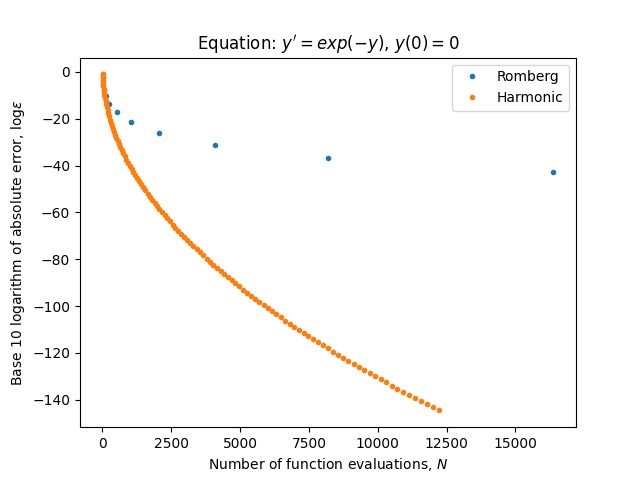
\includegraphics[scale=0.45]{../results/emr_plots/ln_e0_hp.png}
\end{minipage}
\end{figure}

\begin{figure}[H]
\centering
\begin{minipage}{0.45\textwidth}
\centering
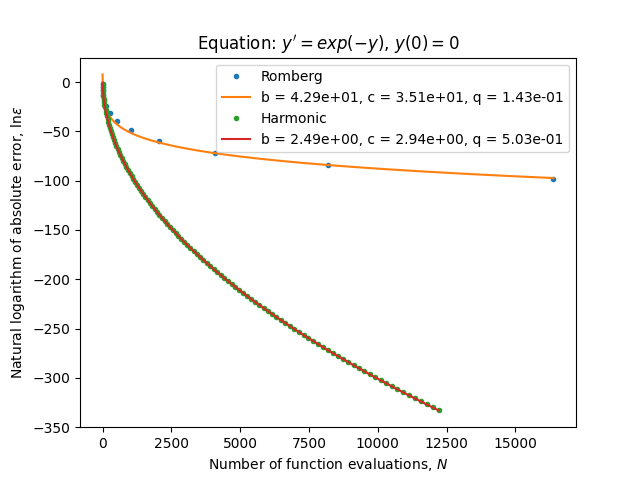
\includegraphics[scale=0.45]{../results/emr_plots/ln_e0_hp_trend.png}
\end{minipage}
\begin{minipage}{0.45\textwidth}
\centering
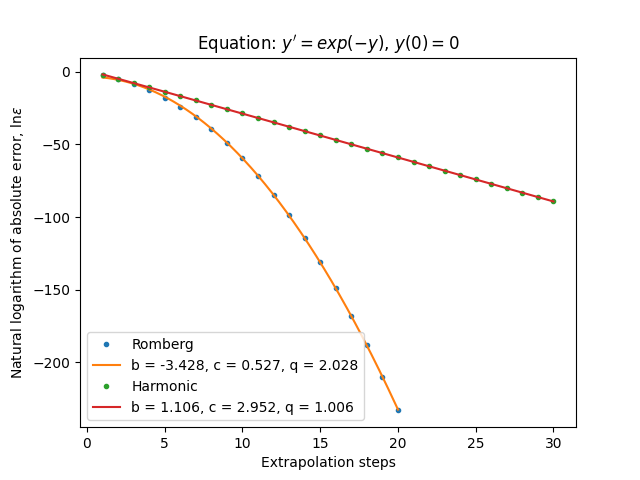
\includegraphics[scale=0.45]{../results/emr_plots/ln_e0_hp_steps.png}
\end{minipage}
\end{figure}

\begin{figure}[H]
\centering
\begin{minipage}{0.45\textwidth}
\centering
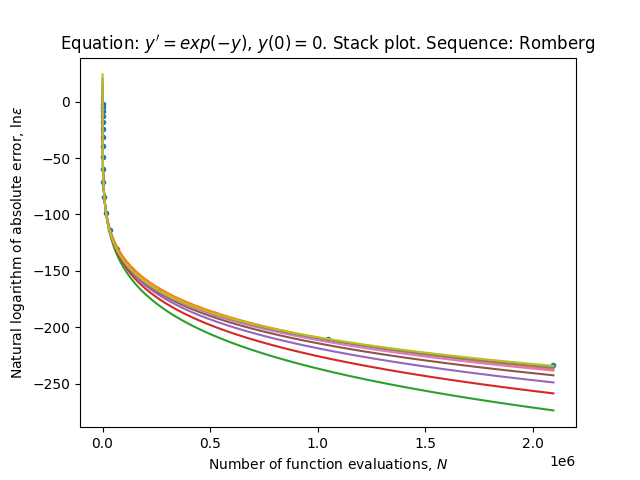
\includegraphics[scale=0.45]{../results/emr_plots/ln_e0_hp_romberg_stack.png}
\end{minipage}
\begin{minipage}{0.45\textwidth}
\centering
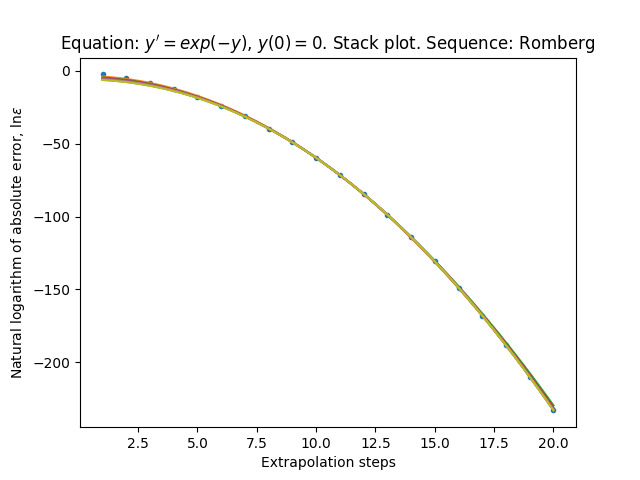
\includegraphics[scale=0.45]{../results/emr_plots/ln_e0_hp_romberg_steps_stack.png}
\end{minipage}
\end{figure}

\begin{figure}[H]
\centering
\begin{minipage}{0.45\textwidth}
\centering
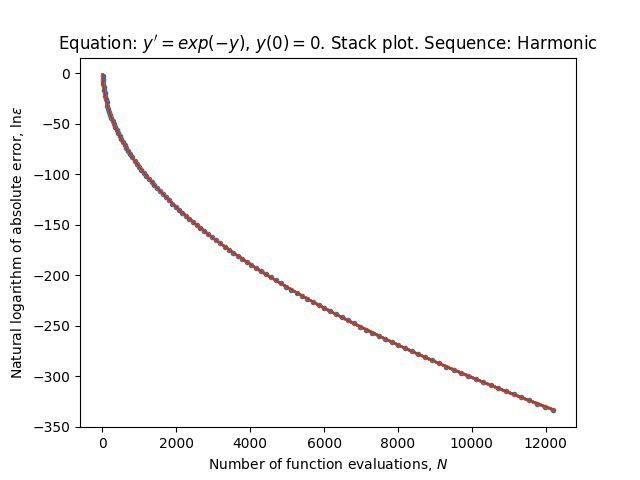
\includegraphics[scale=0.45]{../results/emr_plots/ln_e0_hp_harmonic_stack.png}
\end{minipage}
\begin{minipage}{0.45\textwidth}
\centering
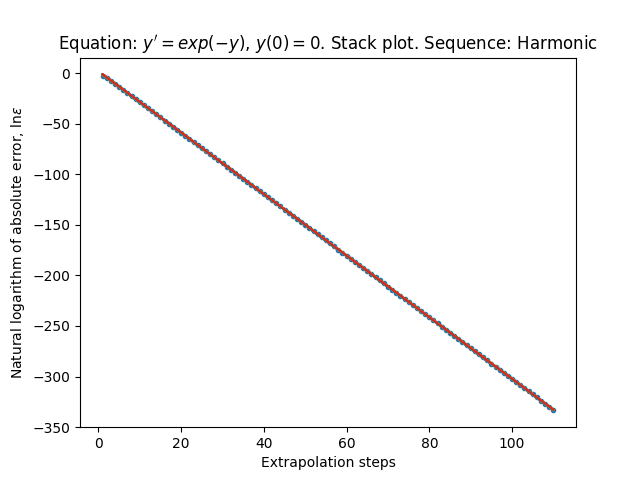
\includegraphics[scale=0.45]{../results/emr_plots/ln_e0_hp_harmonic_steps_stack.png}
\end{minipage}
\end{figure}

\begin{table}[H]
    \centering
    \small
    \begin{tabular}{c||c|c|c|c|c|c|c|c}
Plot & \(A\)-mean & \(A\)-var & \(c\)-mean & \(c\)-var & \(q\)-mean & \(q\)-var & \(\rho_{\operatorname{lin}}\) & \(\rho_{\ln}\)\\\hline
\rowcolor{red}
RS-evals & \(4.9[+42]\) & \(6.0[+00]\) & \(4.5[+01]\) & \(1.2[-01]\) & \(1.4[-01]\) & \(2.8[-02]\) & \(5.2[+05]\) & \(6.0[-04]\) \\
\rowcolor{green}
HS-evals & \(2.1[+01]\) & \(4.2[-02]\) & \(3.0[+00]\) & \(6.2[-05]\) & \(5.0[-01]\) & \(2.7[-06]\) & \(1.3[+00]\) & \(2.9[-07]\) \\
\rowcolor{green}
RS-steps & \(7.5[-03]\) & \(4.1[-01]\) & \(4.8[-01]\) & \(3.3[-03]\) & \(2.1[+00]\) & \(9.1[-05]\) & \(6.0[-01]\) & \(2.1[-05]\) \\
\rowcolor{green}
HS-steps & \(4.9[+00]\) & \(3.5[-02]\) & \(3.0[+00]\) & \(4.9[-05]\) & \(1.0[+00]\) & \(2.1[-06]\) & \(6.7[-01]\) & \(1.9[-07]\) \\
    \end{tabular}
    \label{tab:my_label}
\end{table}

Here the harmonic sequence works better.\\

We have exponential convergence in the number of evaluations and the number of steps for the harmonic sequence and we have exponential convergence in the number of steps for the Romberg sequence.

\subsubsection{\(a = e^{-1}\)}
\begin{figure}[H]
\centering
\begin{minipage}{0.45\textwidth}
\centering
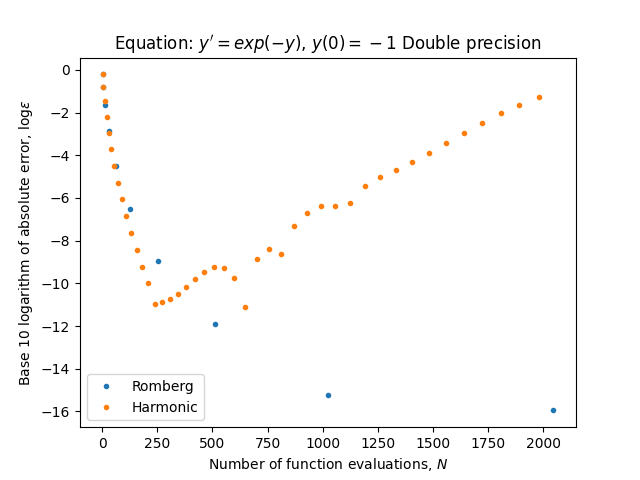
\includegraphics[scale=0.45]{../results/emr_plots/ln_em1.png}
\end{minipage}
\begin{minipage}{0.45\textwidth}
\centering
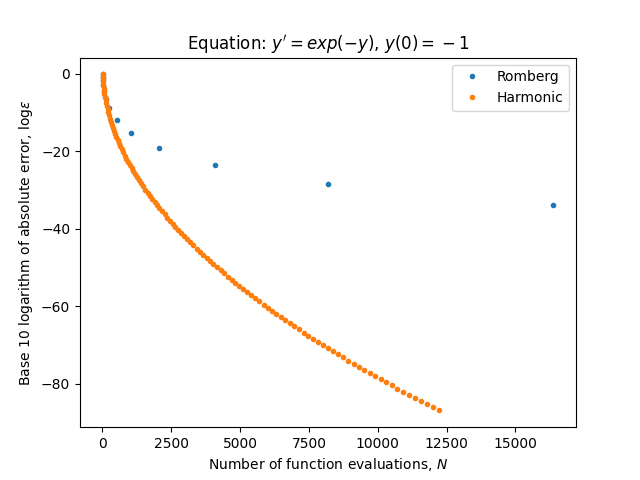
\includegraphics[scale=0.45]{../results/emr_plots/ln_em1_hp.png}
\end{minipage}
\end{figure}

\begin{figure}[H]
\centering
\begin{minipage}{0.45\textwidth}
\centering
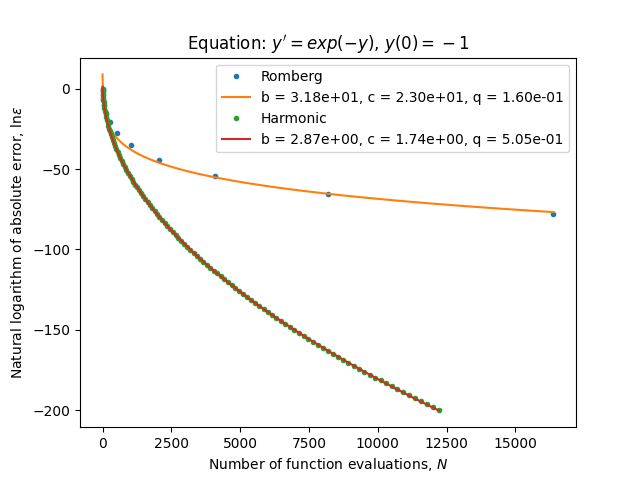
\includegraphics[scale=0.45]{../results/emr_plots/ln_em1_hp_trend.png}
\end{minipage}
\begin{minipage}{0.45\textwidth}
\centering
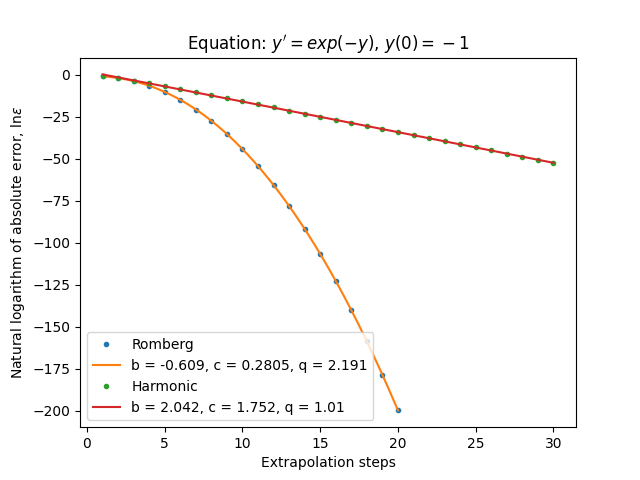
\includegraphics[scale=0.45]{../results/emr_plots/ln_em1_hp_steps.png}
\end{minipage}
\end{figure}

\begin{figure}[H]
\centering
\begin{minipage}{0.45\textwidth}
\centering
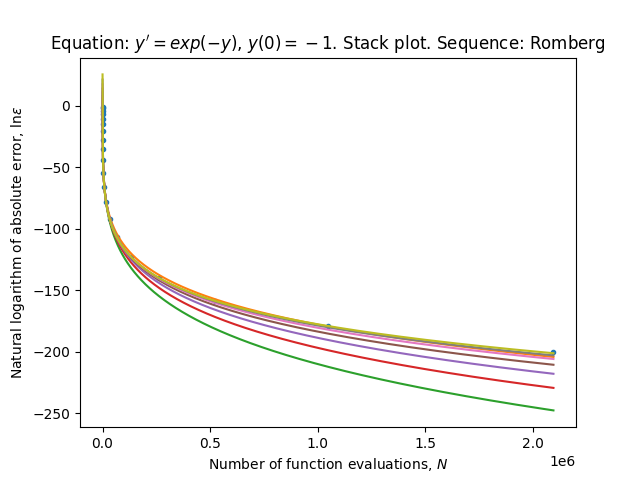
\includegraphics[scale=0.45]{../results/emr_plots/ln_em1_hp_romberg_stack.png}
\end{minipage}
\begin{minipage}{0.45\textwidth}
\centering
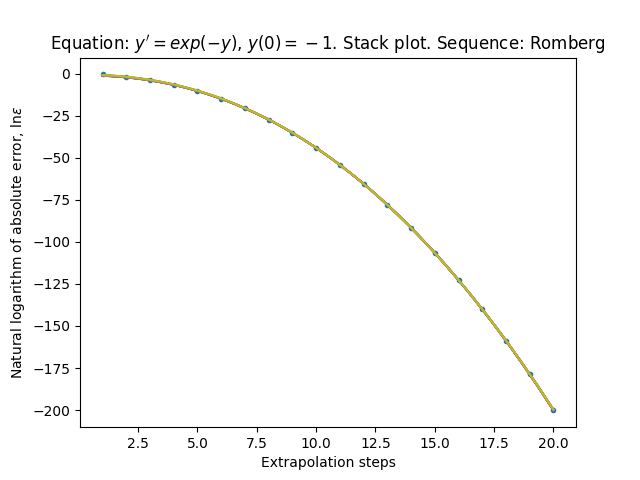
\includegraphics[scale=0.45]{../results/emr_plots/ln_em1_hp_romberg_steps_stack.png}
\end{minipage}
\end{figure}

\begin{figure}[H]
\centering
\begin{minipage}{0.45\textwidth}
\centering
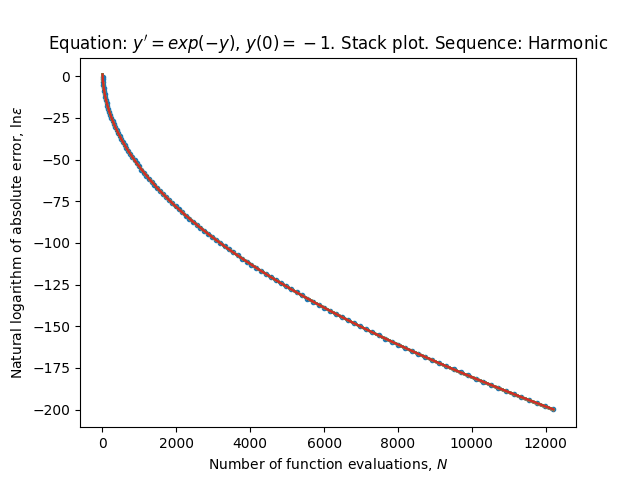
\includegraphics[scale=0.45]{../results/emr_plots/ln_em1_hp_harmonic_stack.png}
\end{minipage}
\begin{minipage}{0.45\textwidth}
\centering
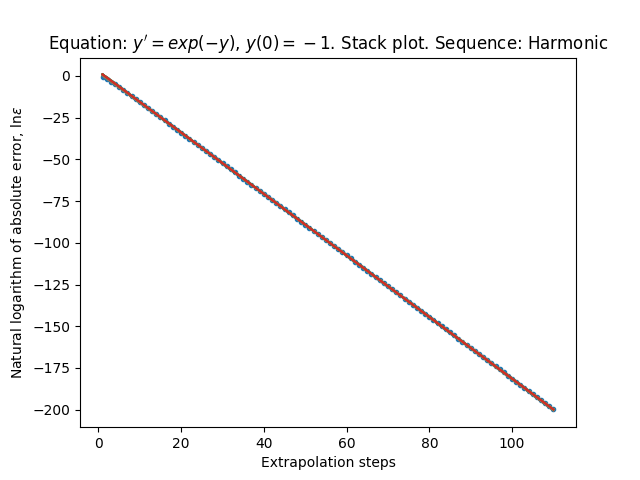
\includegraphics[scale=0.45]{../results/emr_plots/ln_em1_hp_harmonic_steps_stack.png}
\end{minipage}
\end{figure}

\begin{table}[H]
    \centering
    \small
    \begin{tabular}{c||c|c|c|c|c|c|c|c}
Plot & \(A\)-mean & \(A\)-var & \(c\)-mean & \(c\)-var & \(q\)-mean & \(q\)-var & \(\rho_{\operatorname{lin}}\) & \(\rho_{\ln}\)\\\hline
\rowcolor{red}
RS-evals & \(1.3[+34]\) & \(6.0[+00]\) & \(3.0[+01]\) & \(1.6[-01]\) & \(1.5[-01]\) & \(3.4[-02]\) & \(4.9[+05]\) & \(9.1[-04]\) \\
\rowcolor{green}
HS-evals & \(3.1[+01]\) & \(3.6[-02]\) & \(1.8[+00]\) & \(1.3[-04]\) & \(5.0[-01]\) & \(5.8[-06]\) & \(1.9[+00]\) & \(9.4[-07]\) \\
\rowcolor{green}
RS-steps & \(4.2[-01]\) & \(2.5[-02]\) & \(2.7[-01]\) & \(1.9[-04]\) & \(2.2[+00]\) & \(4.2[-06]\) & \(1.0[-01]\) & \(1.7[-06]\) \\
\rowcolor{green}
HS-steps & \(1.3[+01]\) & \(3.1[-02]\) & \(1.8[+00]\) & \(1.1[-04]\) & \(1.0[+00]\) & \(4.9[-06]\) & \(1.3[+00]\) & \(7.4[-07]\) \\
    \end{tabular}
    \label{tab:my_label}
\end{table}

Here the same comments apply as when \(a = 1\).

\subsubsection{\(a = e^{-2}\)}

\begin{figure}[H]
\centering
\begin{minipage}{0.45\textwidth}
\centering
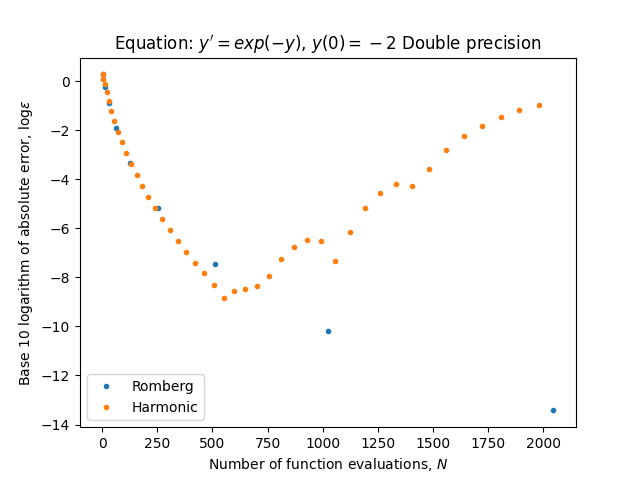
\includegraphics[scale=0.45]{../results/emr_plots/ln_em2.png}
\end{minipage}
\begin{minipage}{0.45\textwidth}
\centering
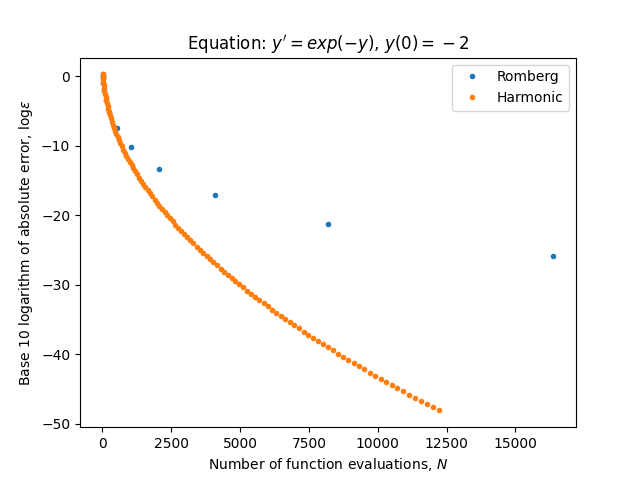
\includegraphics[scale=0.45]{../results/emr_plots/ln_em2_hp.png}
\end{minipage}
\end{figure}

\begin{figure}[H]
\centering
\begin{minipage}{0.45\textwidth}
\centering
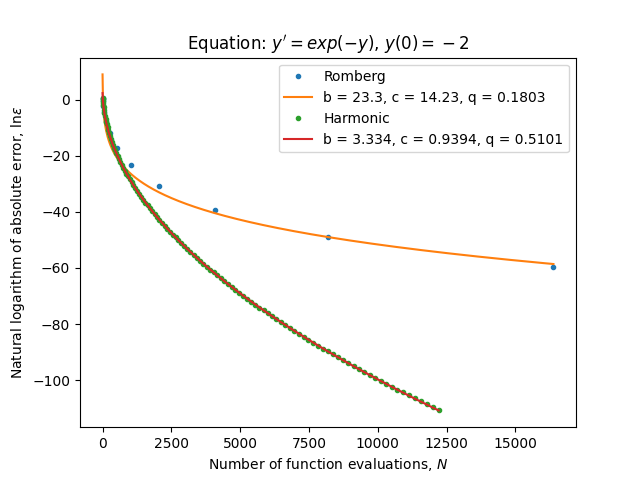
\includegraphics[scale=0.45]{../results/emr_plots/ln_em2_hp_trend.png}
\end{minipage}
\begin{minipage}{0.45\textwidth}
\centering
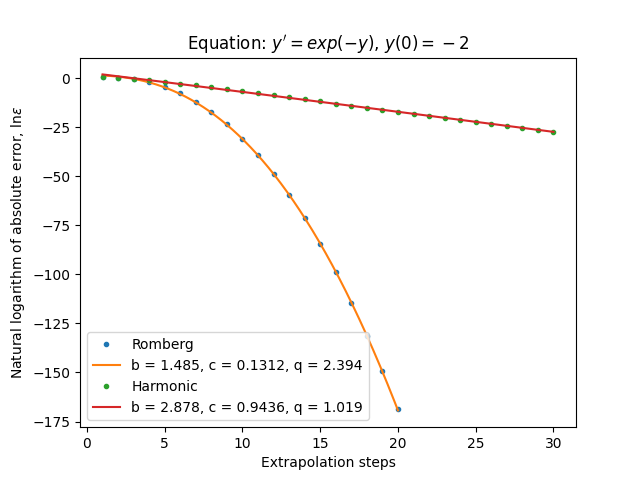
\includegraphics[scale=0.45]{../results/emr_plots/ln_em2_hp_steps.png}
\end{minipage}
\end{figure}

\begin{figure}[H]
\centering
\begin{minipage}{0.45\textwidth}
\centering
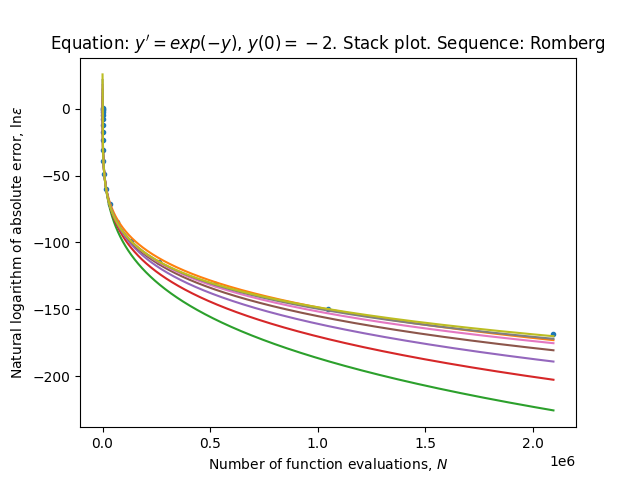
\includegraphics[scale=0.45]{../results/emr_plots/ln_em2_hp_romberg_stack.png}
\end{minipage}
\begin{minipage}{0.45\textwidth}
\centering
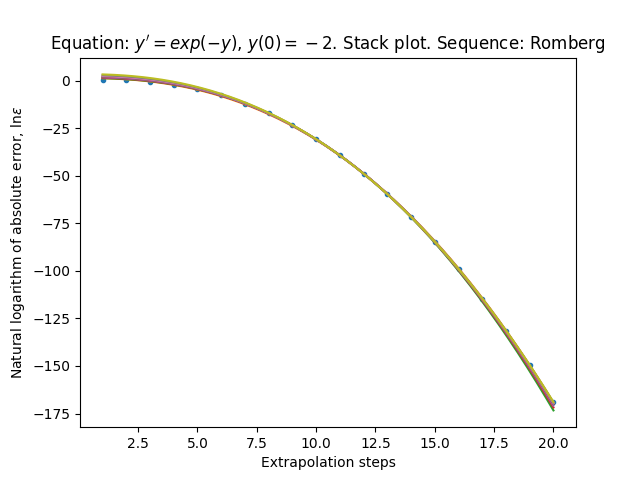
\includegraphics[scale=0.45]{../results/emr_plots/ln_em2_hp_romberg_steps_stack.png}
\end{minipage}
\end{figure}

\begin{figure}[H]
\centering
\begin{minipage}{0.45\textwidth}
\centering
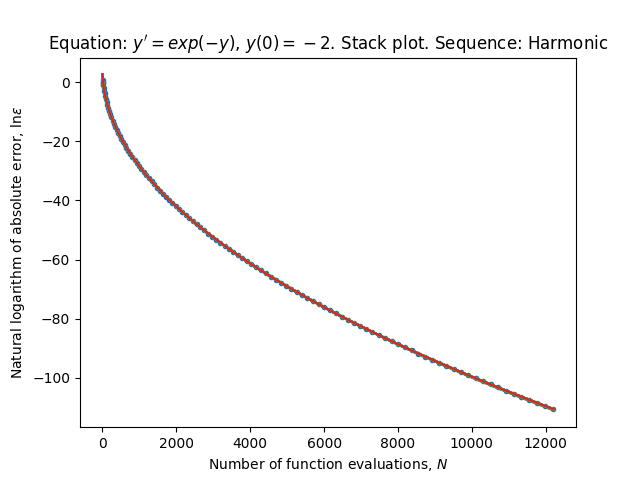
\includegraphics[scale=0.45]{../results/emr_plots/ln_em2_hp_harmonic_stack.png}
\end{minipage}
\begin{minipage}{0.45\textwidth}
\centering
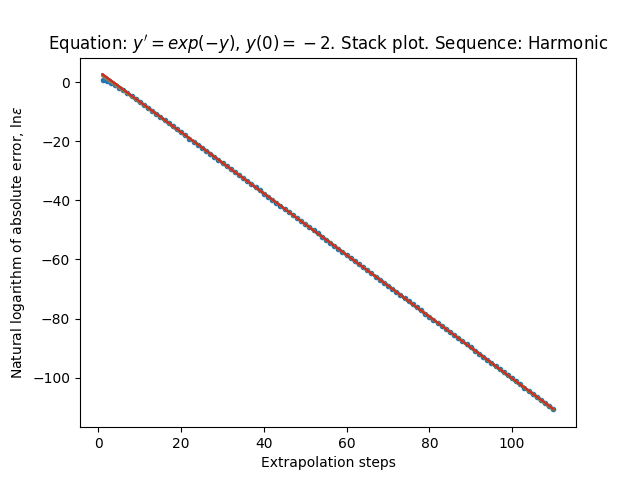
\includegraphics[scale=0.45]{../results/emr_plots/ln_em2_hp_harmonic_steps_stack.png}
\end{minipage}
\end{figure}

\begin{table}[H]
    \centering
    \small
    \begin{tabular}{c||c|c|c|c|c|c|c|c}
Plot & \(A\)-mean & \(A\)-var & \(c\)-mean & \(c\)-var & \(q\)-mean & \(q\)-var & \(\rho_{\operatorname{lin}}\) & \(\rho_{\ln}\)\\\hline
\rowcolor{red}
RS-evals & \(6.7[+26]\) & \(6.0[+00]\) & \(1.9[+01]\) & \(2.2[-01]\) & \(1.8[-01]\) & \(4.1[-02]\) & \(2.9[+05]\) & \(1.4[-03]\) \\
\rowcolor{green}
HS-evals & \(5.3[+01]\) & \(1.5[-02]\) & \(9.9[-01]\) & \(1.4[-04]\) & \(5.0[-01]\) & \(6.0[-06]\) & \(5.0[+00]\) & \(7.7[-06]\) \\
\rowcolor{green}
RS-steps & \(1.4[+01]\) & \(5.1[-01]\) & \(1.4[-01]\) & \(1.0[-02]\) & \(2.4[+00]\) & \(2.2[-04]\) & \(7.7[-01]\) & \(2.1[-05]\) \\
\rowcolor{green}
HS-steps & \(3.2[+01]\) & \(1.3[-02]\) & \(9.9[-01]\) & \(1.2[-04]\) & \(1.0[+00]\) & \(5.1[-06]\) & \(4.2[+00]\) & \(7.1[-06]\) \\
    \end{tabular}
    \label{tab:my_label}
\end{table}

Here the same comments apply as when \(a = 1\).

\subsubsection{\(a = e^{-4}\)}

\begin{figure}[H]
\centering
\begin{minipage}{0.45\textwidth}
\centering
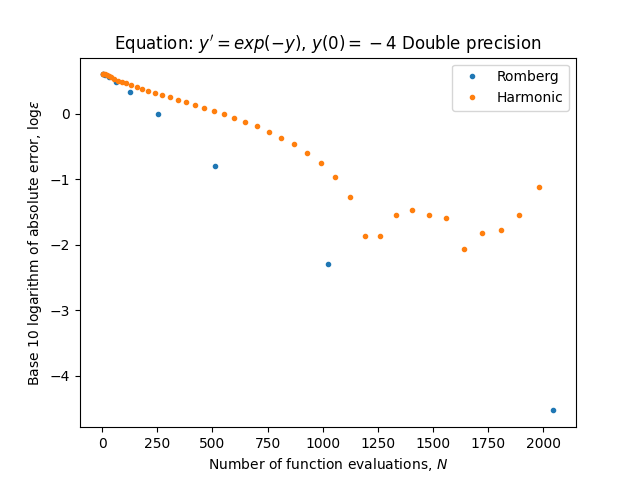
\includegraphics[scale=0.45]{../results/emr_plots/ln_em4.png}
\end{minipage}
\begin{minipage}{0.45\textwidth}
\centering
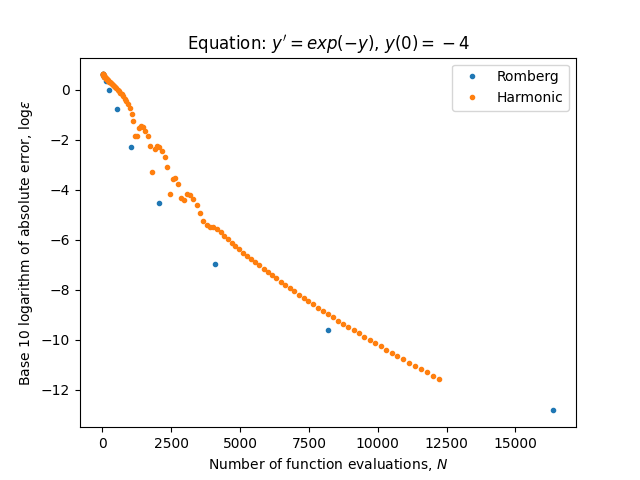
\includegraphics[scale=0.45]{../results/emr_plots/ln_em4_hp.png}
\end{minipage}
\end{figure}

\begin{figure}[H]
\centering
\begin{minipage}{0.45\textwidth}
\centering
\includegraphics[scale=0.45]{../results/emr_plots/ln_em4_hp_trend.png}
\end{minipage}
\begin{minipage}{0.45\textwidth}
\centering
\includegraphics[scale=0.45]{../results/emr_plots/ln_em4_hp_steps.png}
\end{minipage}
\end{figure}

\begin{figure}[H]
\centering
\begin{minipage}{0.45\textwidth}
\centering
\includegraphics[scale=0.45]{../results/emr_plots/ln_em4_hp_romberg_stack.png}
\end{minipage}
\begin{minipage}{0.45\textwidth}
\centering
\includegraphics[scale=0.45]{../results/emr_plots/ln_em4_hp_romberg_steps_stack.png}
\end{minipage}
\end{figure}

\begin{figure}[H]
\centering
\begin{minipage}{0.45\textwidth}
\centering
\includegraphics[scale=0.45]{../results/emr_plots/ln_em4_hp_harmonic_stack.png}
\end{minipage}
\begin{minipage}{0.45\textwidth}
\centering
\includegraphics[scale=0.45]{../results/emr_plots/ln_em4_hp_harmonic_steps_stack.png}
\end{minipage}
\end{figure}

\begin{table}[H]
    \centering
    \small
    \begin{tabular}{c||c|c|c|c|c|c|c|c}
Plot & \(A\)-mean & \(A\)-var & \(c\)-mean & \(c\)-var & \(q\)-mean & \(q\)-var & \(\rho_{\operatorname{lin}}\) & \(\rho_{\ln}\)\\\hline
\rowcolor{red}
RS-evals & \(1.8[+15]\) & \(5.9[+00]\) & \(6.1[+00]\) & \(5.2[-01]\) & \(2.6[-01]\) & \(1.1[-01]\) & \(7.0[+03]\) & \(3.9[-03]\) \\
\rowcolor{red}
HS-evals & \(3.1[+13]\) & \(2.8[+01]\) & \(1.0[+00]\) & \(2.4[+00]\) & \(5.5[-01]\) & \(1.8[-01]\) & \(3.3[+00]\) & \(3.3[-03]\) \\
\rowcolor{red}
RS-steps & \(1.7[+03]\) & \(1.0[+00]\) & \(2.1[-02]\) & \(3.7[-01]\) & \(3.0[+00]\) & \(1.3[-02]\) & \(1.1[+01]\) & \(7.5[-04]\) \\
\rowcolor{red}
HS-steps & \(1.4[+13]\) & \(2.8[+01]\) & \(1.0[+00]\) & \(2.4[+00]\) & \(1.1[+00]\) & \(1.8[-01]\) & \(3.1[+00]\) & \(3.3[-03]\) \\
    \end{tabular}
    \label{tab:my_label}
\end{table}

Here we get much slower convergence than in the previous cases and the model does not fit in any case.

\subsubsection{\(a = e^{-6}\)}

\begin{figure}[H]
\centering
\begin{minipage}{0.45\textwidth}
\centering
\includegraphics[scale=0.45]{../results/emr_plots/ln_em6.png}
\end{minipage}
\begin{minipage}{0.45\textwidth}
\centering
\includegraphics[scale=0.45]{../results/emr_plots/ln_em6_hp.png}
\end{minipage}
\end{figure}

\begin{figure}[H]
\centering
\begin{minipage}{0.45\textwidth}
\centering
\includegraphics[scale=0.45]{../results/emr_plots/ln_em6_hp_trend.png}
\end{minipage}
\begin{minipage}{0.45\textwidth}
\centering
\includegraphics[scale=0.45]{../results/emr_plots/ln_em6_hp_steps.png}
\end{minipage}
\end{figure}

\begin{figure}[H]
\centering
\begin{minipage}{0.45\textwidth}
\centering
\includegraphics[scale=0.45]{../results/emr_plots/ln_em6_hp_romberg_stack.png}
\end{minipage}
\begin{minipage}{0.45\textwidth}
\centering
\includegraphics[scale=0.45]{../results/emr_plots/ln_em6_hp_romberg_steps_stack.png}
\end{minipage}
\end{figure}

\begin{figure}[H]
\centering
\begin{minipage}{0.45\textwidth}
\centering
\includegraphics[scale=0.45]{../results/emr_plots/ln_em6_hp_harmonic_stack.png}
\end{minipage}
\begin{minipage}{0.45\textwidth}
\centering
\includegraphics[scale=0.45]{../results/emr_plots/ln_em6_hp_harmonic_steps_stack.png}
\end{minipage}
\end{figure}

\begin{table}[H]
    \centering
    \small
     \begin{tabular}{c||c|c|c|c|c|c|c|c}
Plot & \(A\)-mean & \(A\)-var & \(c\)-mean & \(c\)-var & \(q\)-mean & \(q\)-var & \(\rho_{\operatorname{lin}}\) & \(\rho_{\ln}\)\\\hline
\rowcolor{red}
RS-evals & \(1.1[+04]\) & \(5.8[+00]\) & \(1.7[-01]\) & \(2.5[+00]\) & \(6.3[-01]\) & \(1.7[-01]\) & \(6.6[+00]\) & \(6.1[-03]\) \\
\rowcolor{red}
HS-evals & \(6.7[+00]\) & \(9.2[-04]\) & \(4.1[-03]\) & \(1.5[-01]\) & \(6.0[-01]\) & \(9.7[-03]\) & \(3.4[-04]\) & \(1.0[-04]\) \\
\rowcolor{red}
RS-steps & \(5.4[+01]\) & \(3.3[+00]\) & \(2.9[-05]\) & \(3.8[+00]\) & \(6.4[+00]\) & \(6.7[-02]\) & \(6.6[-01]\) & \(2.1[-03]\) \\
\rowcolor{red}
HS-steps & \(6.6[+00]\) & \(8.8[-04]\) & \(4.1[-03]\) & \(1.5[-01]\) & \(1.2[+00]\) & \(9.4[-03]\) & \(3.4[-04]\) & \(1.0[-04]\) \\
    \end{tabular}
    \label{tab:my_label}
\end{table}

Here we do simply not get convergence towards the solution and all the models fail.

\subsection{Equation with singularity}

Now we will consider the following initial value problem:
\begin{equation}\label{46}
y'(t) = y^2(t),\quad y(0) = 1/(1+a), \quad t\in [0,1]
\end{equation}

whose solution is 
\[
y(t) = \frac{1}{1-(t-a)}.
\]
The solution is meromorphic with a pole at \(1+a\).

\subsubsection{\(a = 1\)}

\begin{figure}[H]
\centering
\begin{minipage}{0.45\textwidth}
\centering
\includegraphics[scale=0.45]{../results/emr_plots/singularity_0.png}
\end{minipage}
\begin{minipage}{0.45\textwidth}
\centering
\includegraphics[scale=0.45]{../results/emr_plots/singularity_0_hp.png}
\end{minipage}
\end{figure}

\begin{figure}[H]
\centering
\begin{minipage}{0.45\textwidth}
\centering
\includegraphics[scale=0.45]{../results/emr_plots/singularity_0_hp_trend.png}
\end{minipage}
\begin{minipage}{0.45\textwidth}
\centering
\includegraphics[scale=0.45]{../results/emr_plots/singularity_0_hp_steps.png}
\end{minipage}
\end{figure}

\begin{figure}[H]
\centering
\begin{minipage}{0.45\textwidth}
\centering
\includegraphics[scale=0.45]{../results/emr_plots/singularity_0_hp_romberg_stack.png}
\end{minipage}
\begin{minipage}{0.45\textwidth}
\centering
\includegraphics[scale=0.45]{../results/emr_plots/singularity_0_hp_romberg_steps_stack.png}
\end{minipage}
\end{figure}

\begin{figure}[H]
\centering
\begin{minipage}{0.45\textwidth}
\centering
\includegraphics[scale=0.45]{../results/emr_plots/singularity_0_hp_harmonic_stack.png}
\end{minipage}
\begin{minipage}{0.45\textwidth}
\centering
\includegraphics[scale=0.45]{../results/emr_plots/singularity_0_hp_harmonic_steps_stack.png}
\end{minipage}
\end{figure}

\begin{table}[H]
    \centering
    \small
    \begin{tabular}{c||c|c|c|c|c|c|c|c}
Plot & \(A\)-mean & \(A\)-var & \(c\)-mean & \(c\)-var & \(q\)-mean & \(q\)-var & \(\rho_{\operatorname{lin}}\) & \(\rho_{\ln}\)\\\hline
\rowcolor{red}
RS-evals & \(1.4[+42]\) & \(6.0[+00]\) & \(4.2[+01]\) & \(1.4[-01]\) & \(1.4[-01]\) & \(3.2[-02]\) & \(1.7[+06]\) & \(7.7[-04]\) \\
\rowcolor{green}
HS-evals & \(4.4[+02]\) & \(5.2[-01]\) & \(2.7[+00]\) & \(1.3[-03]\) & \(5.1[-01]\) & \(5.5[-05]\) & \(5.2[+01]\) & \(3.6[-06]\) \\
\rowcolor{green}
RS-steps & \(4.2[-02]\) & \(3.0[-02]\) & \(4.3[-01]\) & \(3.0[-04]\) & \(2.1[+00]\) & \(8.2[-06]\) & \(2.8[-01]\) & \(4.7[-06]\) \\
\rowcolor{green}
HS-steps & \(1.0[+02]\) & \(4.9[-01]\) & \(2.8[+00]\) & \(1.2[-03]\) & \(1.0[+00]\) & \(5.0[-05]\) & \(3.4[+01]\) & \(3.2[-06]\) \\
    \end{tabular}
    \label{tab:my_label}
\end{table}

The harmonic sequence performes better and we get almost down to machine level precision using standar double precision floating point arithmetic, with either sequence.\\

We have very nice fit for the exponential convergence in the number of steps for the Romberg sequence and also for the harmonic sequence.

\subsubsection{\(a = 10^{-2}\)}

\begin{figure}[H]
\centering
\begin{minipage}{0.45\textwidth}
\centering
\includegraphics[scale=0.45]{../results/emr_plots/singularity_2.png}
\end{minipage}
\begin{minipage}{0.45\textwidth}
\centering
\includegraphics[scale=0.45]{../results/emr_plots/singularity_2_hp.png}
\end{minipage}
\end{figure}

\begin{figure}[H]
\centering
\begin{minipage}{0.45\textwidth}
\centering
\includegraphics[scale=0.45]{../results/emr_plots/singularity_2_hp_trend.png}
\end{minipage}
\begin{minipage}{0.45\textwidth}
\centering
\includegraphics[scale=0.45]{../results/emr_plots/singularity_2_hp_steps.png}
\end{minipage}
\end{figure}

\begin{figure}[H]
\centering
\begin{minipage}{0.45\textwidth}
\centering
\includegraphics[scale=0.45]{../results/emr_plots/singularity_2_hp_romberg_stack.png}
\end{minipage}
\begin{minipage}{0.45\textwidth}
\centering
\includegraphics[scale=0.45]{../results/emr_plots/singularity_2_hp_romberg_steps_stack.png}
\end{minipage}
\end{figure}

\begin{figure}[H]
\centering
\begin{minipage}{0.45\textwidth}
\centering
\includegraphics[scale=0.45]{../results/emr_plots/singularity_2_hp_harmonic_stack.png}
\end{minipage}
\begin{minipage}{0.45\textwidth}
\centering
\includegraphics[scale=0.45]{../results/emr_plots/singularity_2_hp_harmonic_steps_stack.png}
\end{minipage}
\end{figure}

\begin{table}[H]
    \centering
    \small
    \begin{tabular}{c||c|c|c|c|c|c|c|c}
Plot & \(A\)-mean & \(A\)-var & \(c\)-mean & \(c\)-var & \(q\)-mean & \(q\)-var & \(\rho_{\operatorname{lin}}\) & \(\rho_{\ln}\)\\\hline
\rowcolor{red}
RS-evals & \(1.2[+12]\) & \(6.0[+00]\) & \(2.8[+00]\) & \(7.7[-01]\) & \(3.1[-01]\) & \(8.3[-02]\) & \(4.0[+02]\) & \(3.6[-03]\) \\
\rowcolor{green}
HS-evals & \(1.7[+02]\) & \(1.2[-01]\) & \(4.0[-02]\) & \(8.6[-02]\) & \(6.5[-01]\) & \(2.4[-03]\) & \(9.8[-03]\) & \(1.0[-04]\) \\
\rowcolor{green}
RS-steps & \(3.5[+03]\) & \(2.9[+00]\) & \(5.2[-03]\) & \(6.3[-01]\) & \(3.5[+00]\) & \(9.4[-03]\) & \(1.5[+00]\) & \(5.0[-04]\) \\
\rowcolor{green}
HS-steps & \(1.7[+02]\) & \(1.1[-01]\) & \(4.0[-02]\) & \(8.2[-02]\) & \(1.3[+00]\) & \(2.2[-03]\) & \(8.5[-03]\) & \(9.5[-05]\) \\
    \end{tabular}
    \label{tab:my_label}
\end{table}

Here Romberg works better and we do not attain as high precisison using the harmonic as when using Romberg, in standard double precision arithmetic.\\

Here the model fits moderately well for Romberg sequence, when considering exponential convergence in the number of steps. We also have moderate fit for the harmonic sequence.

\subsubsection{\(a = 10^{-4}\)}

\begin{figure}[H]
\centering
\begin{minipage}{0.45\textwidth}
\centering
\includegraphics[scale=0.45]{../results/emr_plots/singularity_4.png}
\end{minipage}
\begin{minipage}{0.45\textwidth}
\centering
\includegraphics[scale=0.45]{../results/emr_plots/singularity_4_hp.png}
\end{minipage}
\end{figure}

\begin{figure}[H]
\centering
\begin{minipage}{0.45\textwidth}
\centering
\includegraphics[scale=0.45]{../results/emr_plots/singularity_4_hp_trend.png}
\end{minipage}
\begin{minipage}{0.45\textwidth}
\centering
\includegraphics[scale=0.45]{../results/emr_plots/singularity_4_hp_steps.png}
\end{minipage}
\end{figure}

\begin{figure}[H]
\centering
\begin{minipage}{0.45\textwidth}
\centering
\includegraphics[scale=0.45]{../results/emr_plots/singularity_4_hp_romberg_stack.png}
\end{minipage}
\begin{minipage}{0.45\textwidth}
\centering
\includegraphics[scale=0.45]{../results/emr_plots/singularity_4_hp_romberg_steps_stack.png}
\end{minipage}
\end{figure}

\begin{figure}[H]
\centering
\begin{minipage}{0.45\textwidth}
\centering
\includegraphics[scale=0.45]{../results/emr_plots/singularity_4_hp_harmonic_stack.png}
\end{minipage}
\begin{minipage}{0.45\textwidth}
\centering
\includegraphics[scale=0.45]{../results/emr_plots/singularity_4_hp_harmonic_steps_stack.png}
\end{minipage}
\end{figure}


\begin{table}[H]
    \centering
    \small
    \begin{tabular}{c||c|c|c|c|c|c|c|c}
Plot & \(A\)-mean & \(A\)-var & \(c\)-mean & \(c\)-var & \(q\)-mean & \(q\)-var & \(\rho_{\operatorname{lin}}\) & \(\rho_{\ln}\)\\\hline
\rowcolor{red}
RS-evals & \(1.5[+04]\) & \(2.3[-01]\) & \(4.3[-03]\) & \(2.3[+00]\) & \(7.4[-01]\) & \(4.2[-02]\) & \(1.1[-01]\) & \(3.0[-03]\) \\
\rowcolor{yellow}
HS-evals & \(1.0[+04]\) & \(5.5[-09]\) & \(1.7[-04]\) & \(5.8[-05]\) & \(7.5[-01]\) & \(1.2[-06]\) & \(4.2[-10]\) & \(4.8[-12]\) \\
\rowcolor{yellow}
RS-steps & \(1.1[+04]\) & \(2.2[-02]\) & \(2.0[-08]\) & \(3.2[+00]\) & \(7.6[+00]\) & \(6.3[-03]\) & \(1.8[-02]\) & \(8.8[-04]\) \\
\rowcolor{yellow}
HS-steps & \(1.0[+04]\) & \(3.3[-10]\) & \(1.7[-04]\) & \(5.3[-06]\) & \(1.5[+00]\) & \(1.2[-07]\) & \(2.1[-10]\) & \(2.2[-12]\) \\
    \end{tabular}
    \label{tab:my_label}
\end{table}

Here we clearly do not have exponential convergence in the number of evaluations for the Romberg sequence. We have not so good fit for exponential convergence in the number of steps.\\

Regarding the harmonic sequence, we note that we have extremely slow convergence, so the \(x\) and \(y\) values differ by many orders of magnitude, so the results are maybe not so reliable.

\subsection{Equation with moderate singularity}

Now we will consider the following initial value problem
\begin{equation}
y'(t) = -\frac{1}{2y}, \quad y(0) = \sqrt{1+a},\quad t\in [0,1]\label{47}
\end{equation}
whose solution is 
\[
y(t) = \sqrt{1 - (t-a)}
\]

\subsubsection{\(a = 1\)}

\begin{figure}[H]
\centering
\begin{minipage}{0.45\textwidth}
\centering
\includegraphics[scale=0.45]{../results/emr_plots/quad_sing_0.png}
\end{minipage}
\begin{minipage}{0.45\textwidth}
\centering
\includegraphics[scale=0.45]{../results/emr_plots/quad_sing_0_hp.png}
\end{minipage}
\end{figure}

\begin{figure}[H]
\centering
\begin{minipage}{0.45\textwidth}
\centering
\includegraphics[scale=0.45]{../results/emr_plots/quad_sing_0_hp_trend.png}
\end{minipage}
\begin{minipage}{0.45\textwidth}
\centering
\includegraphics[scale=0.45]{../results/emr_plots/quad_sing_0_hp_steps.png}
\end{minipage}
\end{figure}

\begin{figure}[H]
\centering
\begin{minipage}{0.45\textwidth}
\centering
\includegraphics[scale=0.45]{../results/emr_plots/quad_sing_0_hp_romberg_stack.png}
\end{minipage}
\begin{minipage}{0.45\textwidth}
\centering
\includegraphics[scale=0.45]{../results/emr_plots/quad_sing_0_hp_romberg_steps_stack.png}
\end{minipage}
\end{figure}

\begin{figure}[H]
\centering
\begin{minipage}{0.45\textwidth}
\centering
\includegraphics[scale=0.45]{../results/emr_plots/quad_sing_0_hp_harmonic_stack.png}
\end{minipage}
\begin{minipage}{0.45\textwidth}
\centering
\includegraphics[scale=0.45]{../results/emr_plots/quad_sing_0_hp_harmonic_steps_stack.png}
\end{minipage}
\end{figure}

\begin{table}[H]
    \centering
    \small
    \begin{tabular}{c||c|c|c|c|c|c|c|c}
Plot & \(A\)-mean & \(A\)-var & \(c\)-mean & \(c\)-var & \(q\)-mean & \(q\)-var & \(\rho_{\operatorname{lin}}\) & \(\rho_{\ln}\)\\\hline
\rowcolor{red}
RS-evals & \(8.3[+41]\) & \(6.0[+00]\) & \(4.7[+01]\) & \(1.1[-01]\) & \(1.3[-01]\) & \(2.6[-02]\) & \(1.5[+05]\) & \(4.9[-04]\) \\
\rowcolor{green}
HS-evals & \(4.5[-01]\) & \(3.6[-02]\) & \(3.1[+00]\) & \(3.8[-05]\) & \(5.0[-01]\) & \(1.6[-06]\) & \(6.8[-02]\) & \(7.0[-08]\) \\
\rowcolor{green}
RS-steps & \(2.8[-04]\) & \(7.4[-01]\) & \(5.1[-01]\) & \(5.8[-03]\) & \(2.0[+00]\) & \(1.6[-04]\) & \(7.9[-01]\) & \(4.0[-05]\) \\
\rowcolor{green}
HS-steps & \(1.0[-01]\) & \(4.1[-02]\) & \(3.1[+00]\) & \(4.4[-05]\) & \(1.0[+00]\) & \(1.9[-06]\) & \(1.3[-01]\) & \(1.2[-07]\) \\
    \end{tabular}
    \label{tab:my_label}
\end{table}

Here the harmonic sequence works better than Romberg and we get down to machine level precision using either sequence, in standard double precision floating point arithmetic.\\

Here we clearly have exponential convergence in the number of steps and evaluations for the harmonic sequence. Regarding Romberg, we seem to have exponential convergence in the number of steps.

\subsubsection{\(a = 10^{-2}\)}

\begin{figure}[H]
\centering
\begin{minipage}{0.45\textwidth}
\centering
\includegraphics[scale=0.45]{../results/emr_plots/quad_sing_2.png}
\end{minipage}
\begin{minipage}{0.45\textwidth}
\centering
\includegraphics[scale=0.45]{../results/emr_plots/quad_sing_2_hp.png}
\end{minipage}
\end{figure}

\begin{figure}[H]
\centering
\begin{minipage}{0.45\textwidth}
\centering
\includegraphics[scale=0.45]{../results/emr_plots/quad_sing_2_hp_trend.png}
\end{minipage}
\begin{minipage}{0.45\textwidth}
\centering
\includegraphics[scale=0.45]{../results/emr_plots/quad_sing_2_hp_steps.png}
\end{minipage}
\end{figure}

\begin{figure}[H]
\centering
\begin{minipage}{0.45\textwidth}
\centering
\includegraphics[scale=0.45]{../results/emr_plots/quad_sing_2_hp_romberg_stack.png}
\end{minipage}
\begin{minipage}{0.45\textwidth}
\centering
\includegraphics[scale=0.45]{../results/emr_plots/quad_sing_2_hp_romberg_steps_stack.png}
\end{minipage}
\end{figure}

\begin{figure}[H]
\centering
\begin{minipage}{0.45\textwidth}
\centering
\includegraphics[scale=0.45]{../results/emr_plots/quad_sing_2_hp_harmonic_stack.png}
\end{minipage}
\begin{minipage}{0.45\textwidth}
\centering
\includegraphics[scale=0.45]{../results/emr_plots/quad_sing_2_hp_harmonic_steps_stack.png}
\end{minipage}
\end{figure}

\begin{table}[H]
    \centering
    \small
    \begin{tabular}{c||c|c|c|c|c|c|c|c}
Plot & \(A\)-mean & \(A\)-var & \(c\)-mean & \(c\)-var & \(q\)-mean & \(q\)-var & \(\rho_{\operatorname{lin}}\) & \(\rho_{\ln}\)\\\hline
\rowcolor{red}
RS-evals & \(3.1[+09]\) & \(6.0[+00]\) & \(4.5[+00]\) & \(4.3[-01]\) & \(2.5[-01]\) & \(4.6[-02]\) & \(1.7[+02]\) & \(1.4[-03]\) \\
\rowcolor{green}
HS-evals & \(9.3[-02]\) & \(5.5[-02]\) & \(2.6[-01]\) & \(1.1[-02]\) & \(4.8[-01]\) & \(4.5[-04]\) & \(2.3[-01]\) & \(5.1[-05]\) \\
\rowcolor{green}
RS-steps & \(2.1[-01]\) & \(1.2[+00]\) & \(1.4[-02]\) & \(1.1[-01]\) & \(3.0[+00]\) & \(1.3[-03]\) & \(1.7[-01]\) & \(5.7[-05]\) \\
\rowcolor{green}
HS-steps & \(8.3[-02]\) & \(5.0[-02]\) & \(2.6[-01]\) & \(1.1[-02]\) & \(9.6[-01]\) & \(4.4[-04]\) & \(2.3[-01]\) & \(5.1[-05]\) \\
    \end{tabular}
    \label{tab:my_label}
\end{table}

Here Romberg performes better and we do not attain as high precision using the harmonic sequence in standard double precision floating point arithmetic.\\

For the Romberg sequence, the model seems to fit moderately well when considering exponential convergence in the number of evaluations. We also have reasonably good fit for the harmonic sequence.\\

\subsubsection{\(a = 10^{-4}\)}

\begin{figure}[H]
\centering
\begin{minipage}{0.45\textwidth}
\centering
\includegraphics[scale=0.45]{../results/emr_plots/quad_sing_4.png}
\end{minipage}
\begin{minipage}{0.45\textwidth}
\centering
\includegraphics[scale=0.45]{../results/emr_plots/quad_sing_4_hp.png}
\end{minipage}
\end{figure}

\begin{figure}[H]
\centering
\begin{minipage}{0.45\textwidth}
\centering
\includegraphics[scale=0.45]{../results/emr_plots/quad_sing_4_hp_trend.png}
\end{minipage}
\begin{minipage}{0.45\textwidth}
\centering
\includegraphics[scale=0.45]{../results/emr_plots/quad_sing_4_hp_steps.png}
\end{minipage}
\end{figure}

\begin{figure}[H]
\centering
\begin{minipage}{0.45\textwidth}
\centering
\includegraphics[scale=0.45]{../results/emr_plots/quad_sing_4_hp_romberg_stack.png}
\end{minipage}
\begin{minipage}{0.45\textwidth}
\centering
\includegraphics[scale=0.45]{../results/emr_plots/quad_sing_4_hp_romberg_steps_stack.png}
\end{minipage}
\end{figure}

\begin{figure}[H]
\centering
\begin{minipage}{0.45\textwidth}
\centering
\includegraphics[scale=0.45]{../results/emr_plots/quad_sing_4_hp_harmonic_stack.png}
\end{minipage}
\begin{minipage}{0.45\textwidth}
\centering
\includegraphics[scale=0.45]{../results/emr_plots/quad_sing_4_hp_harmonic_steps_stack.png}
\end{minipage}
\end{figure}

\begin{table}[H]
    \centering
    \small
    \begin{tabular}{c||c|c|c|c|c|c|c|c}
Plot & \(A\)-mean & \(A\)-var & \(c\)-mean & \(c\)-var & \(q\)-mean & \(q\)-var & \(\rho_{\operatorname{lin}}\) & \(\rho_{\ln}\)\\\hline
\rowcolor{red}
RS-evals & \(1.4[-01]\) & \(4.8[-01]\) & \(2.5[-01]\) & \(4.6[-01]\) & \(3.5[-01]\) & \(1.9[-02]\) & \(1.7[-01]\) & \(4.5[-04]\) \\
\rowcolor{red}
HS-evals & \(1.3[+00]\) & \(3.4[+00]\) & \(1.3[+00]\) & \(3.9[-01]\) & \(1.6[-01]\) & \(5.5[-02]\) & \(1.2[-02]\) & \(4.9[-05]\) \\
\rowcolor{red}
RS-steps & \(4.3[-02]\) & \(5.1[-01]\) & \(1.8[-03]\) & \(3.8[+00]\) & \(4.0[+00]\) & \(4.4[-02]\) & \(4.7[-01]\) & \(1.8[-03]\) \\
\rowcolor{red}
HS-steps & \(8.1[-01]\) & \(1.7[+00]\) & \(1.1[+00]\) & \(3.1[-01]\) & \(3.3[-01]\) & \(4.6[-02]\) & \(7.4[-03]\) & \(3.5[-05]\) \\
    \end{tabular}
    \label{tab:my_label}
\end{table}

Here, we do not have any clear fit.

\subsection{Circular rotation}

Now we will consider the following system of equations:
\begin{equation}\label{48}
(y_1(t),y_2(t))' = (-y_2(t), y_1(t)), \quad y(0) = (1,0), \quad t\in [0,\pi /2]
\end{equation}
whose solution is 
\[
(y_1(t),y_2(t)) = (\cos t, \sin t)
\]
which is entire.

\begin{figure}[H]
\centering
\begin{minipage}{0.45\textwidth}
\centering
\includegraphics[scale=0.45]{../results/emr_plots/rotation.png}
\end{minipage}
\begin{minipage}{0.45\textwidth}
\centering
\includegraphics[scale=0.45]{../results/emr_plots/rotation_hp.png}
\end{minipage}
\end{figure}

\begin{figure}[H]
\centering
\begin{minipage}{0.45\textwidth}
\centering
\includegraphics[scale=0.45]{../results/emr_plots/rotation_hp_trend.png}
\end{minipage}
\begin{minipage}{0.45\textwidth}
\centering
\includegraphics[scale=0.45]{../results/emr_plots/rotation_hp_steps.png}
\end{minipage}
\end{figure}

\begin{figure}[H]
\centering
\begin{minipage}{0.45\textwidth}
\centering
\includegraphics[scale=0.45]{../results/emr_plots/rotation_hp_romberg_stack.png}
\end{minipage}
\begin{minipage}{0.45\textwidth}
\centering
\includegraphics[scale=0.45]{../results/emr_plots/rotation_hp_romberg_steps_stack.png}
\end{minipage}
\end{figure}

\begin{figure}[H]
\centering
\begin{minipage}{0.45\textwidth}
\centering
\includegraphics[scale=0.45]{../results/emr_plots/rotation_hp_harmonic_stack.png}
\end{minipage}
\begin{minipage}{0.45\textwidth}
\centering
\includegraphics[scale=0.45]{../results/emr_plots/rotation_hp_harmonic_steps_stack.png}
\end{minipage}
\end{figure}

\begin{table}[H]
    \centering
    \small
    \begin{tabular}{c||c|c|c|c|c|c|c|c}
Plot & \(A\)-mean & \(A\)-var & \(c\)-mean & \(c\)-var & \(q\)-mean & \(q\)-var & \(\rho_{\operatorname{lin}}\) & \(\rho_{\ln}\)\\\hline
\rowcolor{red}
RS-evals & \(1.2[+60]\) & \(6.0[+00]\) & \(6.1[+01]\) & \(1.4[-01]\) & \(1.3[-01]\) & \(3.5[-02]\) & \(2.3[+08]\) & \(8.6[-04]\) \\
\rowcolor{green}
HS-evals & \(9.0[+09]\) & \(6.8[+00]\) & \(2.6[+00]\) & \(7.9[-03]\) & \(6.2[-01]\) & \(2.5[-04]\) & \(4.4[+05]\) & \(8.9[-06]\) \\
\rowcolor{green}
RS-steps & \(1.1[+00]\) & \(1.0[-04]\) & \(6.7[-01]\) & \(5.0[-07]\) & \(2.0[+00]\) & \(1.5[-08]\) & \(2.9[-03]\) & \(2.0[-08]\) \\
\rowcolor{green}
HS-steps & \(4.3[+08]\) & \(6.5[+00]\) & \(2.7[+00]\) & \(6.9[-03]\) & \(1.2[+00]\) & \(2.2[-04]\) & \(9.5[+04]\) & \(7.5[-06]\) \\
    \end{tabular}
    \label{tab:my_label}
\end{table}

The harmonic sequence works better then Romberg and we get down to machine level precision using either sequence when using standard floating point arithmetic.\\

We clearly have exponential convergence in the number of steps for the Romberg sequence. For the harmonic sequence, we seem to have exponential convergence, but though we must note that the mean value of the \(A\) coefficient is quite large.

\subsection{Mathematical pendulum}

Now we will consider the mathematical pendulum equation:
\begin{equation}
y''(t) + \sin y(t) = 0,\quad y(0) = 0,\, y'(0) = 1, \quad t\in [0,1].
\end{equation}

\begin{figure}[H]
\centering
\includegraphics[scale=0.6]{../results/trajectories/mathematical_pendulum_trajectory.png}
\end{figure}

Here we computed a reference solution up to \(500\) digits which can be found in the code.\\

\begin{figure}[H]
\centering
\begin{minipage}{0.45\textwidth}
\centering
\includegraphics[scale=0.45]{../results/emr_plots/oscillation.png}
\end{minipage}
\begin{minipage}{0.45\textwidth}
\centering
\includegraphics[scale=0.45]{../results/emr_plots/oscillation_hp.png}
\end{minipage}
\end{figure}

\begin{figure}[H]
\centering
\begin{minipage}{0.45\textwidth}
\centering
\includegraphics[scale=0.45]{../results/emr_plots/oscillation_hp_trend.png}
\end{minipage}
\begin{minipage}{0.45\textwidth}
\centering
\includegraphics[scale=0.45]{../results/emr_plots/oscillation_hp_steps.png}
\end{minipage}
\end{figure}

\begin{figure}[H]
\centering
\begin{minipage}{0.45\textwidth}
\centering
\includegraphics[scale=0.45]{../results/emr_plots/oscillation_hp_romberg_stack.png}
\end{minipage}
\begin{minipage}{0.45\textwidth}
\centering
\includegraphics[scale=0.45]{../results/emr_plots/oscillation_hp_romberg_steps_stack.png}
\end{minipage}
\end{figure}

\begin{figure}[H]
\centering
\begin{minipage}{0.45\textwidth}
\centering
\includegraphics[scale=0.45]{../results/emr_plots/oscillation_hp_harmonic_stack.png}
\end{minipage}
\begin{minipage}{0.45\textwidth}
\centering
\includegraphics[scale=0.45]{../results/emr_plots/oscillation_hp_harmonic_steps_stack.png}
\end{minipage}
\end{figure}

\begin{table}[H]
    \centering
    \small
    \begin{tabular}{c||c|c|c|c|c|c|c|c}
Plot & \(A\)-mean & \(A\)-var & \(c\)-mean & \(c\)-var & \(q\)-mean & \(q\)-var & \(\rho_{\operatorname{lin}}\) & \(\rho_{\ln}\)\\\hline
\rowcolor{red}
RS-evals & \(3.2[+52]\) & \(6.0[+00]\) & \(5.7[+01]\) & \(1.4[-01]\) & \(1.3[-01]\) & \(3.9[-02]\) & \(1.4[+06]\) & \(5.6[-04]\) \\
\rowcolor{green}
HS-evals & \(4.7[+0]\) & \(2.7[-01]\) & \(3.7[+00]\) & \(2.6[-04]\) & \(5.0[-01]\) & \(1.1[-05]\) & \(9.6[+00]\) & \(1.1[-06]\) \\
\rowcolor{green}
RS-steps & \(1.4[-02]\) & \(3.3[-01]\) & \(6.3[-01]\) & \(2.1[-03]\) & \(2.0[+00]\) & \(6.2[-05]\) & \(6.7[-01]\) & \(2.8[-05]\) \\
\rowcolor{green}
HS-steps & \(7.3[+01]\) & \(2.5[-01]\) & \(3.7[+00]\) & \(2.3[-04]\) & \(1.0[+00]\) & \(9.9[-06]\) & \(5.2[+00]\) & \(9.2[-07]\) \\
    \end{tabular}
    \label{tab:my_label}
\end{table}

Here the harmonic sequence works better and we get down to machine level precision in standard double precision floating point arithmetic, using either sequence.\\

We have nice fit for the exponential convergence in the number of steps for the Romberg sequence. We also have very nice fit for the harmonic sequence.

\subsection{Federpendel}

Now we will consider the equation of motion for das Federpendel or the spring pendulum:
\[
\bfp' = -(|\bfq| - 1)\frac{\bfq}{|\bfq|} - {1\choose 0}, \quad \bfq' = \bfp
\]
where \(\bfp\) and \(\bfq\) are two dimensional vectors. We will consider it with the initial condition \(\bfq(0) = (1,0)\) and \(\bfp(0) = (0,1)\) and try to both estimate the solution at times \(t = 1\), \(t = 2\) and \(t=10\).\\

In the first two cases we use precomputed solutions with accurracy of \(500\) digits and in the third case we use a solution with accurracy of \(250\) digits. The solutions can be found in the code.

\begin{figure}[H]
\centering
\includegraphics[scale=0.6]{../results/trajectories/federpendel_trajectory.png}
\end{figure}

\subsubsection{\(t = 1\)}

Here we use a reference solution which was computed 

\begin{figure}[H]
\centering
\begin{minipage}{0.45\textwidth}
\centering
\includegraphics[scale=0.45]{../results/emr_plots/federpendel.png}
\end{minipage}
\begin{minipage}{0.45\textwidth}
\centering
\includegraphics[scale=0.45]{../results/emr_plots/federpendel_1_hp.png}
\end{minipage}
\end{figure}

\begin{figure}[H]
\centering
\begin{minipage}{0.45\textwidth}
\centering
\includegraphics[scale=0.45]{../results/emr_plots/federpendel_1_hp_trend.png}
\end{minipage}
\begin{minipage}{0.45\textwidth}
\centering
\includegraphics[scale=0.45]{../results/emr_plots/federpendel_1_hp_steps.png}
\end{minipage}
\end{figure}

\begin{figure}[H]
\centering
\begin{minipage}{0.45\textwidth}
\centering
\includegraphics[scale=0.45]{../results/emr_plots/federpendel_1_hp_romberg_stack.png}
\end{minipage}
\begin{minipage}{0.45\textwidth}
\centering
\includegraphics[scale=0.45]{../results/emr_plots/federpendel_1_hp_romberg_steps_stack.png}
\end{minipage}
\end{figure}

\begin{figure}[H]
\centering
\begin{minipage}{0.45\textwidth}
\centering
\includegraphics[scale=0.45]{../results/emr_plots/federpendel_1_hp_harmonic_stack.png}
\end{minipage}
\begin{minipage}{0.45\textwidth}
\centering
\includegraphics[scale=0.45]{../results/emr_plots/federpendel_1_hp_harmonic_steps_stack.png}
\end{minipage}
\end{figure}

\begin{table}[H]
    \centering
    \small
    \begin{tabular}{c||c|c|c|c|c|c|c|c}
Plot & \(A\)-mean & \(A\)-var & \(c\)-mean & \(c\)-var & \(q\)-mean & \(q\)-var & \(\rho_{\operatorname{lin}}\) & \(\rho_{\ln}\)\\\hline
\rowcolor{red}
RS-evals & \(8.2[+40]\) & \(6.0[+00]\) & \(4.4[+01]\) & \(1.2[-01]\) & \(1.4[-01]\) & \(2.8[-02]\) & \(3.1[+05]\) & \(5.4[-04]\) \\
\rowcolor{green}
HS-evals & \(5.1[-01]\) & \(2.5[-01]\) & \(2.6[+00]\) & \(3.4[-04]\) & \(5.0[-01]\) & \(1.5[-05]\) & \(2.7[-01]\) & \(1.8[-06]\) \\
\rowcolor{green}
RS-steps & \(2.8[-03]\) & \(3.7[-01]\) & \(4.6[-01]\) & \(3.3[-03]\) & \(2.1[+00]\) & \(8.9[-05]\) & \(6.5[-01]\) & \(3.7[-05]\) \\
\rowcolor{green}
HS-steps & \(1.5[-01]\) & \(2.5[-01]\) & \(2.6[+00]\) & \(3.5[-04]\) & \(9.9[-01]\) & \(1.5[-05]\) & \(3.2[-01]\) & \(2.0[-06]\) \\
    \end{tabular}
    \label{tab:my_label}
\end{table}

Here the harmonic sequence works better and we get down to machine level precision in standard double precision floating point arithmetic, using either sequence.\\

We have nice fit for exponential convergence in the number of steps for the Romberg sequence. We also have nice fit for exponential convergence for the harmonic sequence.

\subsubsection{\(t = 2\)}

Here we use \(1\) as initial step length.

\begin{figure}[H]
\centering
\begin{minipage}{0.45\textwidth}
\centering
\includegraphics[scale=0.45]{../results/emr_plots/federpendel_2.png}
\end{minipage}
\begin{minipage}{0.45\textwidth}
\centering
\includegraphics[scale=0.45]{../results/emr_plots/federpendel_2_hp.png}
\end{minipage}
\end{figure}

\begin{figure}[H]
\centering
\begin{minipage}{0.45\textwidth}
\centering
\includegraphics[scale=0.45]{../results/emr_plots/federpendel_2_hp_trend.png}
\end{minipage}
\begin{minipage}{0.45\textwidth}
\centering
\includegraphics[scale=0.45]{../results/emr_plots/federpendel_2_hp_steps.png}
\end{minipage}
\end{figure}

\begin{figure}[H]
\centering
\begin{minipage}{0.45\textwidth}
\centering
\includegraphics[scale=0.45]{../results/emr_plots/federpendel_2_hp_romberg_stack.png}
\end{minipage}
\begin{minipage}{0.45\textwidth}
\centering
\includegraphics[scale=0.45]{../results/emr_plots/federpendel_2_hp_romberg_steps_stack.png}
\end{minipage}
\end{figure}

\begin{figure}[H]
\centering
\begin{minipage}{0.45\textwidth}
\centering
\includegraphics[scale=0.45]{../results/emr_plots/federpendel_2_hp_harmonic_stack.png}
\end{minipage}
\begin{minipage}{0.45\textwidth}
\centering
\includegraphics[scale=0.45]{../results/emr_plots/federpendel_2_hp_harmonic_steps_stack.png}
\end{minipage}
\end{figure}

\begin{table}[H]
    \centering
    \small
    \begin{tabular}{c||c|c|c|c|c|c|c|c}
Plot & \(A\)-mean & \(A\)-var & \(c\)-mean & \(c\)-var & \(q\)-mean & \(q\)-var & \(\rho_{\operatorname{lin}}\) & \(\rho_{\ln}\)\\\hline
\rowcolor{red}
RS-evals & \(6.5[+39]\) & \(6.0[+00]\) & \(4.2[+01]\) & \(1.2[-01]\) & \(1.4[-01]\) & \(2.7[-02]\) & \(4.0[+05]\) & \(6.0[-04]\) \\
\rowcolor{green}
HS-evals & \(4.2[-01]\) & \(3.7[-01]\) & \(2.4[+00]\) & \(5.1[-04]\) & \(4.9[-01]\) & \(2.2[-05]\) & \(1.8[-01]\) & \(1.3[-06]\) \\
\rowcolor{green}
RS-steps & \(5.0[-03]\) & \(4.6[-01]\) & \(4.4[-01]\) & \(4.0[-03]\) & \(2.1[+00]\) & \(1.1[-04]\) & \(5.6[-01]\) & \(2.2[-05]\) \\
\rowcolor{green}
HS-steps & \(1.3[-01]\) & \(3.6[-01]\) & \(2.4[+00]\) & \(5.2[-04]\) & \(9.9[-01]\) & \(2.2[-05]\) & \(2.3[-01]\) & \(1.5[-06]\) \\
    \end{tabular}
    \label{tab:my_label}
\end{table}

Here the harmonic sequence also works better and we attain high precision using either sequence in standard double precision floating point arithmetic.\\

We seem to have very nice fit for exponential convergence in the number of steps for the Romberg sequence. We also have very nice fit for exponential convergence for the harmonic sequence.

\subsubsection{\(t = 10\)}

Here we use \(1\) as initial step length. When too big initial step length was used, the convergence failed. Hence the results are dependent upon the initial step length. 

\begin{figure}[H]
\centering
\begin{minipage}{0.45\textwidth}
\centering
\includegraphics[scale=0.45]{../results/emr_plots/federpendel_10.png}
\end{minipage}
\begin{minipage}{0.45\textwidth}
\centering
\includegraphics[scale=0.45]{../results/emr_plots/federpendel_10_hp.png}
\end{minipage}
\end{figure}

\begin{figure}[H]
\centering
\begin{minipage}{0.45\textwidth}
\centering
\includegraphics[scale=0.45]{../results/emr_plots/federpendel_10_hp_trend.png}
\end{minipage}
\begin{minipage}{0.45\textwidth}
\centering
\includegraphics[scale=0.45]{../results/emr_plots/federpendel_10_hp_steps.png}
\end{minipage}
\end{figure}

\begin{figure}[H]
\centering
\begin{minipage}{0.45\textwidth}
\centering
\includegraphics[scale=0.45]{../results/emr_plots/federpendel_10_hp_romberg_stack.png}
\end{minipage}
\begin{minipage}{0.45\textwidth}
\centering
\includegraphics[scale=0.45]{../results/emr_plots/federpendel_10_hp_romberg_steps_stack.png}
\end{minipage}
\end{figure}

\begin{figure}[H]
\centering
\begin{minipage}{0.45\textwidth}
\centering
\includegraphics[scale=0.45]{../results/emr_plots/federpendel_10_hp_harmonic_stack.png}
\end{minipage}
\begin{minipage}{0.45\textwidth}
\centering
\includegraphics[scale=0.45]{../results/emr_plots/federpendel_10_hp_harmonic_steps_stack.png}
\end{minipage}
\end{figure}

\begin{table}[H]
    \centering
    \small
    \begin{tabular}{c||c|c|c|c|c|c|c|c}
Plot & \(A\)-mean & \(A\)-var & \(c\)-mean & \(c\)-var & \(q\)-mean & \(q\)-var & \(\rho_{\operatorname{lin}}\) & \(\rho_{\ln}\)\\\hline
\rowcolor{red}
RS-evals & \(1.9[+50]\) & \(6.0[+00]\) & \(4.3[+01]\) & \(2.0[-01]\) & \(1.4[-01]\) & \(3.0[-02]\) & \(6.4[+05]\) & \(7.4[-04]\) \\
\rowcolor{green}
HS-evals & \(3.9[+00]\) & \(3.9[+00]\) & \(1.9[+00]\) & \(1.1[-02]\) & \(4.9[-01]\) & \(4.6[-04]\) & \(6.0[-01]\) & \(1.2[-05]\) \\
\rowcolor{green}
RS-steps & \(9.7[-01]\) & \(4.8[+00]\) & \(4.4[-01]\) & \(4.0[-02]\) & \(2.1[+00]\) & \(1.1[-03]\) & \(4.4[-01]\) & \(2.7[-05]\) \\
\rowcolor{green}
HS-steps & \(1.6[+00]\) & \(3.9[+00]\) & \(1.9[+00]\) & \(1.1[-02]\) & \(9.8[-01]\) & \(4.6[-04]\) & \(6.3[-01]\) & \(1.2[-05]\) \\
    \end{tabular}
    \label{tab:my_label}
\end{table}

Here we still have exponential convergence in the number of steps for both sequences.

\subsection{Lorenz equations}

The Lorenz equations are the following system: 
\[
\frac{dx}{dt} = \sigma (y-x),\quad \frac{dy}{dt} = x(\rho - z) - y,\quad \frac{dz}{dt} = xy - \beta z
\]
where \(\sigma,\,\rho\) and \(\beta\) are constants. In our experiment, the constants are set to \(\sigma = 10\), \(\rho = 28\) and \(\beta = 8/3\). The initial condition we will consider is \((x(0),y(0),z(0)) = (1,1,1)\).\\

We use precomputed reference solutions with accurracy of \(500\) digits which can be found in the code.

\subsubsection{\(t = 0.1\)}

\begin{figure}[H]
\centering
\begin{minipage}{0.45\textwidth}
\centering
\includegraphics[scale=0.45]{../results/emr_plots/lorenz.png}
\end{minipage}
\begin{minipage}{0.45\textwidth}
\centering
\includegraphics[scale=0.45]{../results/emr_plots/lorenz_hp.png}
\end{minipage}
\end{figure}

\begin{figure}[H]
\centering
\begin{minipage}{0.45\textwidth}
\centering
\includegraphics[scale=0.45]{../results/emr_plots/lorenz_hp_trend.png}
\end{minipage}
\begin{minipage}{0.45\textwidth}
\centering
\includegraphics[scale=0.45]{../results/emr_plots/lorenz_hp_steps.png}
\end{minipage}
\end{figure}

\begin{figure}[H]
\centering
\begin{minipage}{0.45\textwidth}
\centering
\includegraphics[scale=0.45]{../results/emr_plots/lorenz_hp_romberg_stack.png}
\end{minipage}
\begin{minipage}{0.45\textwidth}
\centering
\includegraphics[scale=0.45]{../results/emr_plots/lorenz_hp_romberg_steps_stack.png}
\end{minipage}
\end{figure}

\begin{figure}[H]
\centering
\begin{minipage}{0.45\textwidth}
\centering
\includegraphics[scale=0.45]{../results/emr_plots/lorenz_hp_harmonic_stack.png}
\end{minipage}
\begin{minipage}{0.45\textwidth}
\centering
\includegraphics[scale=0.45]{../results/emr_plots/lorenz_hp_harmonic_steps_stack.png}
\end{minipage}
\end{figure}

\begin{table}[H]
    \centering\small
    \begin{tabular}{c||c|c|c|c|c|c|c|c}
Plot & \(A\)-mean & \(A\)-var & \(c\)-mean & \(c\)-var & \(q\)-mean & \(q\)-var & \(\rho_{\operatorname{lin}}\) & \(\rho_{\ln}\)\\\hline
\rowcolor{red}
RS-evals & \(1.5[+73]\) & \(6.0[+00]\) & \(6.6[+01]\) & \(2.6[-01]\) & \(1.3[-01]\) & \(7.3[-02]\) & \(5.8[+08]\) & \(1.2[-03]\) \\
\rowcolor{green}
HS-evals & \(2.6[+07]\) & \(6.8[+00]\) & \(4.2[+00]\) & \(1.8[-03]\) & \(5.1[-01]\) & \(7.2[-05]\) & \(9.2[+05]\) & \(2.2[-05]\) \\
\rowcolor{green}
RS-steps & \(8.9[+03]\) & \(2.3[+00]\) & \(7.2[-01]\) & \(6.4[-02]\) & \(2.0[+00]\) & \(2.0[-03]\) & \(4.0[+00]\) & \(3.6[-05]\) \\
\rowcolor{green}
HS-steps & \(2.9[+06]\) & \(6.6[+00]\) & \(4.2[+00]\) & \(1.8[-03]\) & \(1.0[+00]\) & \(7.1[-05]\) & \(5.4[+05]\) & \(2.1[-05]\) \\
    \end{tabular}
    \label{tab:my_label}
\end{table}

Here the harmonic sequence works better and we get down to machine level precision in standard double precision arithmetic.\\

The model for exponential convergence in the number of steps fits moderately well for the Romberg sequence. We get nice fit for exponential convergence for the harmonic sequence.

\subsubsection{\(t = 0.2\)}

Here we use \(0.1\) as initial step length. 

\begin{figure}[H]
\centering
\begin{minipage}{0.45\textwidth}
\centering
\includegraphics[scale=0.45]{../results/emr_plots/lorenz_02.png}
\end{minipage}
\begin{minipage}{0.45\textwidth}
\centering
\includegraphics[scale=0.45]{../results/emr_plots/lorenz_02_hp.png}
\end{minipage}
\end{figure}

\begin{figure}[H]
\centering
\begin{minipage}{0.45\textwidth}
\centering
\includegraphics[scale=0.45]{../results/emr_plots/lorenz_02_hp_trend.png}
\end{minipage}
\begin{minipage}{0.45\textwidth}
\centering
\includegraphics[scale=0.45]{../results/emr_plots/lorenz_02_hp_steps.png}
\end{minipage}
\end{figure}

\begin{figure}[H]
\centering
\begin{minipage}{0.45\textwidth}
\centering
\includegraphics[scale=0.45]{../results/emr_plots/lorenz_02_hp_romberg_stack.png}
\end{minipage}
\begin{minipage}{0.45\textwidth}
\centering
\includegraphics[scale=0.45]{../results/emr_plots/lorenz_02_hp_romberg_steps_stack.png}
\end{minipage}
\end{figure}

\begin{figure}[H]
\centering
\begin{minipage}{0.45\textwidth}
\centering
\includegraphics[scale=0.45]{../results/emr_plots/lorenz_02_hp_harmonic_stack.png}
\end{minipage}
\begin{minipage}{0.45\textwidth}
\centering
\includegraphics[scale=0.45]{../results/emr_plots/lorenz_02_hp_harmonic_steps_stack.png}
\end{minipage}
\end{figure}

\begin{table}[H]
    \centering
    \small
    \begin{tabular}{c||c|c|c|c|c|c|c|c}
Plot & \(A\)-mean & \(A\)-var & \(c\)-mean & \(c\)-var & \(q\)-mean & \(q\)-var & \(\rho_{\operatorname{lin}}\) & \(\rho_{\ln}\)\\\hline
\rowcolor{red}
RS-evals & \(3.8[+53]\) & \(6.0[+00]\) & \(5.0[+01]\) & \(1.6[-01]\) & \(1.4[-01]\) & \(3.8[-02]\) & \(2.0[+08]\) & \(1.1[-03]\) \\
\rowcolor{green}
HS-evals & \(6.3[+08]\) & \(7.6[+00]\) & \(4.0[+00]\) & \(1.5[-02]\) & \(5.0[-01]\) & \(5.8[-04]\) & \(9.5[+05]\) & \(2.3[-05]\) \\
\rowcolor{green}
RS-steps & \(6.1[+01]\) & \(1.6[-01]\) & \(5.2[-01]\) & \(1.3[-03]\) & \(2.1[+00]\) & \(3.8[-05]\) & \(1.5[+00]\) & \(7.0[-06]\) \\
\rowcolor{green}
HS-steps & \(7.3[+07]\) & \(7.5[+00]\) & \(4.0[+00]\) & \(1.5[-02]\) & \(1.0[+00]\) & \(5.7[-04]\) & \(6.0[+05]\) & \(2.2[-05]\) \\
    \end{tabular}
    \label{tab:my_label}
\end{table}

Here we also get down to machine level precision in standard double precision floating point arithmetic. The harmonic sequence performes better.\\

The model for exponential convergence in the number of steps fits moderately well for the Romberg sequence. We get moderate fit for exponential convergence for the harmonic sequence.

\section{Summary}

When the solutions are entire we seem to have exponential convergence in the number of steps for both the Romberg sequence and the harmonic sequence. The same holds when the solutions are analytic and we are not too close to a singularity. When we move closer to the singularities, the fitting becomes worse and the convergence begins to fail.\\

It is interesting how fast convergence we get with the harmonic sequence when computing nicely behaved solutions.\\

It would be interesting to analyze further how the convergence depends on the initial step size.\\